\documentclass[a4paper, 12pt]{article}
\usepackage[utf8]{vietnam}
\usepackage[english]{babel}
\usepackage{graphicx}
\usepackage{color}
\usepackage{fancyhdr}
\usepackage{array}
\usepackage{geometry}
\usepackage{enumitem}
\usepackage{blindtext}
\usepackage{tabularx}
\usepackage[table,xcdraw]{xcolor}
\usepackage{makecell}
\setcounter{tocdepth}{5}
\usepackage{titlesec}
\usepackage{tocloft}
\usepackage{adjustbox}
\usepackage{xcolor} 
\usepackage{tikz}
\usepackage{float}
\usepackage{hyperref}
\usepackage{csquotes}
\usepackage{array}
\hypersetup{
    colorlinks=true,
    linkcolor=black,
    filecolor=magenta,
    citecolor=blue,
    urlcolor=blue,
}
\usepackage{supertabular}
\usepackage{biblatex}
\addbibresource{ref.bib}

\geometry{
    a4paper,
    total={170mm,257mm},
    left=20mm,
    top=20mm,
}
\usepackage{lipsum}
\usepackage{multicol}
\usepackage[svgnames,table]{xcolor}
\usepackage{minted}
\definecolor{LightGray}{gray}{0.9}
\usepackage{amsmath}
\begin{document}

\thispagestyle{empty}
\begin{titlepage}
            \begin{tikzpicture}[remember picture,overlay,inner sep=0,outer sep=0]
        \draw[blue!70!black,line width=4pt] ([xshift=-1.5cm,yshift=-2cm]current page.north east) coordinate (A)--([xshift=1.5cm,yshift=-2cm]current page.north west) coordinate(B)--([xshift=1.5cm,yshift=2cm]current page.south west) coordinate (C)--([xshift=-1.5cm,yshift=2cm]current page.south east) coordinate(D)--cycle;

        \draw ([yshift=0.5cm,xshift=-0.5cm]A)-- ([yshift=0.5cm,xshift=0.5cm]B)--
        ([yshift=-0.5cm,xshift=0.5cm]B) --([yshift=-0.5cm,xshift=-0.5cm]B)--([yshift=0.5cm,xshift=-0.5cm]C)--([yshift=0.5cm,xshift=0.5cm]C)--([yshift=-0.5cm,xshift=0.5cm]C)-- ([yshift=-0.5cm,xshift=-0.5cm]D)--([yshift=0.5cm,xshift=-0.5cm]D)--([yshift=0.5cm,xshift=0.5cm]D)--([yshift=-0.5cm,xshift=0.5cm]A)--([yshift=-0.5cm,xshift=-0.5cm]A)--([yshift=0.5cm,xshift=-0.5cm]A);


        \draw ([yshift=-0.3cm,xshift=0.3cm]A)-- ([yshift=-0.3cm,xshift=-0.3cm]B)--
        ([yshift=0.3cm,xshift=-0.3cm]B) --([yshift=0.3cm,xshift=0.3cm]B)--([yshift=-0.3cm,xshift=0.3cm]C)--([yshift=-0.3cm,xshift=-0.3cm]C)--([yshift=0.3cm,xshift=-0.3cm]C)-- ([yshift=0.3cm,xshift=0.3cm]D)--([yshift=-0.3cm,xshift=0.3cm]D)--([yshift=-0.3cm,xshift=-0.3cm]D)--([yshift=0.3cm,xshift=-0.3cm]A)--([yshift=0.3cm,xshift=0.3cm]A)--([yshift=-0.3cm,xshift=0.3cm]A);
    \end{tikzpicture}
	\begin{center}
        VIET NAM NATIONAL UNIVERSITY - HO CHI MINH CITY\\
		UNIVERSITY OF SCIENCE \\
		FACULTY OF INFORMATION TECHNOLOGY
	\end{center}
	\begin{figure}[h!]
		\begin{center}
			
\includegraphics[width=8cm]{logo KHTN.png}
		\end{center}
	\end{figure}
	\begin{center}
		\begin{tabular}{c}
			\multicolumn{1}{c}{\textbf{{\LARGE DATA STRUCTURES AND ALGORITHMS}}} \\
			~~                                                                 \\
			\\
			\hline
			\\
			\multicolumn{1}{c}{\textbf{{\Huge REPORT}}}                       \\
			\\
			\textbf{{\huge STATIC HUFFMAN COMPRESSION}}                              \\
			\\
			\hline
		\end{tabular}
	\end{center}
    \begin{center}
        \textbf{\large{GROUP 4}}\\[0.5cm]

        \begin{table}[H]
            \begin{center}
                \begin{tabular}{rrrlc}
                     & \large{\textbf{Theory Lecturer}} & \large{Dr.} & \large{Nguyen Thanh Phuong}        &                  \\
                     & \large{\textbf{Lab Lecturer}}    & \large{Dr.} &\large{Nguyen Ngoc Thao} &                  \\
                     &                                  & \large{M.S.} & \large{Nguyen Thanh Tinh} &                  \\
                     &                                  &                              &                  \\
                     & \large{\textbf{Students}}        & \large{24127104} & \large{Du Hoai Phuc - Leader}          \\
                     &                                  & \large{24127008} & \large{Truong Nhat Phat}\\
                     &                                  & \large{24127173} & \large{Nguyen Tuan Hung}
                \end{tabular}
            \end{center}
        \end{table}
    \end{center}
	\vspace{3cm}
\end{titlepage}

\tableofcontents
% Header and Footer
\pagestyle{fancy}
\lhead{\tikz[baseline=(X.base)] \node[fill=cyan!80!blue, text=white, font=\bfseries, rounded corners=5pt, inner sep=5pt] (X) {Data structures and Algorithms};}
\rhead{\textbf{Static Huffman compression}}
\lfoot{\textbf{Group 4 | Class 24C06}}
\cfoot{}
\rfoot{\tikz[baseline=(X.base)] \node[fill=cyan!80!blue, text=white, font=\bfseries, rounded corners=10pt, inner sep=10pt] (X) {\thepage};}
\setlength{\headheight}{24pt}
\setlength{\footskip}{30pt}
% Đổi màu cho đường kẻ header và footer
\renewcommand{\headrulewidth}{2pt}
\renewcommand{\footrulewidth}{2pt}
\renewcommand{\headrule}{\hbox to\headwidth{\color{cyan}\leaders\hrule height \headrulewidth\hfill}}
\renewcommand{\footrule}{\hbox to\headwidth{\color{cyan}\leaders\hrule height \footrulewidth\hfill}}
% Thêm dấu chấm sau mỗi section
\renewcommand{\cftsecaftersnum}{.}
\renewcommand{\cftsubsecaftersnum}{.}

\cftsetindents{section}{0em}{2em}
\cftsetindents{subsection}{2em}{2em}
\cftsetindents{subsubsection}{4em}{1em}
\cftsetindents{paragraph}{3.5em}{1em}
\cftsetindents{subparagraph}{4em}{1em}

\titleformat{\paragraph}[block]{\normalfont\normalsize\bfseries}{\theparagraph}{0.5em}{}
\titleformat{\subparagraph}[block]{\normalfont\normalsize\bfseries}{\theparagraph}{0.5em}{}
\newpage
\pagenumbering{arabic}

%Thông tin nhóm
\section*{General information}

\subsection*{Member's information:}
\begin{center}
	\begin{table}[H]
		\renewcommand{\arraystretch}{1.5}
		\setlength{\tabcolsep}{8pt} % Giảm khoảng cách giữa các cột để tiết kiệm không gian
		\rowcolors{2}{gray!15}{white}
		\resizebox{\textwidth}{!}{ % Tự động co bảng vừa chiều rộng trang
			\begin{tabular}{|c|l|l|l|}
				\hline
				\rowcolor{gray!30}
				\textbf{ID} & \textbf{Full name}   & \textbf{Email}               & \textbf{Roles}                \\
				\hline
				24127104                 & Du Hoai Phuc         & dhphuc2424@clc.fitus.edu.vn  & Leader, Report Editor        \\
				24127173                 & Nguyen Tuan Hung     & nthung2432@clc.fitus.edu.vn  & Data Analysis, Code Optimizer \\
				24127008                 & Truong Nhat Phat     & tnphat2418@clc.fitus.edu.vn  & Algorithm Analysis, Editor        \\
				\hline
			\end{tabular}}
		\caption{Group's information}
	\end{table}
\end{center}


\subsection*{Task assignment}
\begin{center}
\begin{table}[H]
    \renewcommand{\arraystretch}{1.5}
    \setlength{\tabcolsep}{8pt} % Giảm khoảng cách giữa các cột để tiết kiệm không gian
    \rowcolors{2}{gray!15}{white}
    \resizebox{\textwidth}{!}{ % Tự động co bảng vừa chiều rộng trang
        \begin{tabular}{|c|l|l|c|}
            \hline
            \rowcolor{gray!30}
            \textbf{No.} & \textbf{Task}   & \textbf{Assignee}               & \textbf{Progress}                \\
            \hline
            1                 & Coding         & Nguyen Tuan Hung  & 100\%       \\
            2                 & Introduction to Compression & Nguyen Tuan Hung & 100\% \\
            3                 & Introduction to Huffman Coding     & Truong Nhat Phat  & 100\% \\
            4                 & Algorithm Theory     & Truong Nhat Phat  & 100\% \\
            5                 & Algorithm Visualization    & Du Hoai Phuc  & 100\%        \\
            6                 & Algorithm variances     & Truong Nhat Phat  & 100\% \\
            7                 & Performance Experiment     & Nguyen Tuan Hung  & 100\% \\
            8                 & Pros and Cons     & Nguyen Tuan Hung  & 100\% \\
            9                 & Discover the Application of Algorithm    & Truong Nhat Phat  & 100\% \\
            10                & Compare with other compression Algorithms     & Nguyen Tuan Hung  & 100\% \\
            11                 & Check progress      & Du Hoai Phuc  & 100\% \\
            12                 & Report combination    & Du Hoai Phuc  & 100\% \\
            13                 & Record description    & Du Hoai Phuc  & 100\% \\
            14                 & Report editing    & Du Hoai Phuc  & 100\% \\
            15                 & Video editing     & Truong Nhat Phat  & 100\% \\
            16                 & Slide             & Du Hoai Phuc & 100\% \\
            \hline
        \end{tabular}}
    \caption{Task assignment}
\end{table}
\end{center}

\newpage

% Trật tự trình bày:
% 1. Introduction to Compression: Giới thiệu tổng quan về nén dữ liệu.
% 2. Introduction to Huffman Coding: Giới thiệu về mã hóa Huffman.
% 3. Algorithm Theory: Chi tiết thuật toán.
% 4. Algorithm Visualization: Minh họa thuật toán.
% 5. Algorithm Variances: Các biến thể của thuật toán.
% 6. Performance Experiment: Thí nghiệm hiệu suất.
% 7. Pros and Cons: Ưu và nhược điểm của thuật toán.
% 8. Discover the Application of Algorithm: Khám phá ứng dụng của thuật toán.
% 9. Compare with other Compression Algorithms: So sánh với các thuật toán nén khác. 

\section{Introduction to Compression}
\subsection{Overview of Compression}
Data is a crucial part of the digital world, representing information in various forms such as text, images, audio, and video. It serves as the backbone of modern computing, communication, analysis, and decision-making across several industries. The rapid growth of data in recent years, has led to the development of advanced storage, processing, and compression techniques to optimize efficiency and accessibility. Proper data management is essential for ensuring security, accuracy, and usability in applications ranging from AI to cloud computing.\newline
Data compression is a type of data management that helps reduce the size of data without (or with minimal) loss of information. In the era of G.AI where a large amount of data can be generated in a blink of an eye, data compression is not just desirable but an absolute necessity.
\subsection{History of Compression}
The history of data compression dates back to the early days of computing, driven by the need to store and transmit data efficiently since the storage device and bandwidth are limited resources. One of the first cases of data compression is Morse code which assigns shorter code to frequent use letters. In 1948, Claude Shannon laid the foundation for data compression with their groundbreaking work on information theory, introducing the concept of entropy and establishing the theoretical limits on lossless compression. In 1952, Huffman Coding was introduced by David A. Huffman, an optimal algorithm for generating prefix-free, variable-length codes. The 1970s and 80s brought the Lempel-Ziv family of algorithms (LZ77, LZ78, and LZW), which introduced dictionary-based methods and became widely adopted in various applications. The 1990s saw the rise of JPEG and MP3, which introduced lossy compression techniques for images and audio, balancing quality and file size. Today, data compression research continues to advance, exploring areas like deep learning-based compression and specialized algorithms for emerging data types, reflecting the ongoing quest to manage the ever-expanding volume of digital information.
\subsection{Type of Compression}
Data compression techniques can be broadly classified into two fundamental categories: lossless and lossy compression.
\begin{itemize}
    \item \textbf{Lossless Compression}: These techniques guarantee perfect reconstruction of the original data after decompression. No information is lost in the process. Lossless compression is essential for applications where data integrity is paramount, such as text documents, executable files, and medical images. Examples include Run-Length Encoding (RLE), Huffman Coding, and the Lempel-Ziv family of algorithms.
    \item \textbf{Lossy Compression}: These techniques achieve higher compression ratios by discarding some information that is deemed less important or imperceptible. The decompressed data is an approximation of the original, but the loss is often acceptable in applications like image, audio, and video streaming, where minor imperfections are tolerable. Examples include JPEG for images, MP3 for audio, and MPEG for video.
\end{itemize}
Another distinction is between symmetric and asymmetric compression. Symmetric compression algorithms have similar computational complexity for both encoding and decoding, while asymmetric algorithms have significantly different complexities (typically, encoding is much more complex than decoding).
\subsection{Lossless Compression}
\begin{enumerate}[label=\textbf{\Alph*.}]
    \item \textbf{Run-Length Encoding (RLE)} \begin{itemize}
        \item Basic principles: replacing sequences of identical data with a count and the repeated value.
        \item Example: "AAAAABBBCC" -> "5A3B2C"
        \item Application: Simple images, fax, text with repetitive patterns.
        \item Advantages: Simple, fast.
        \item Disadvantages: Not effective for data with little repetition.
    \end{itemize}
    \item \textbf{Huffman Coding} \begin{itemize}
        \item Basic principle: variable-length codes based on symbol frequencies (shorter codes for more frequent symbols).
        \item Example: "BEEBE BEE" -> 0111011000111 (in bit representation)
        \item Application: JPEG, MP3, GZIP, general-purpose compression.
        \item Advantages: Optimal for symbol-by-symbol encoding, widely used.
        \item Disadvantages: Requires frequency information (static) or adaptation (adaptive).
    \end{itemize}
    \item \textbf{Arithmetic Coding} \begin{itemize}
        \item Principle: Encodes the entire message as a single fraction within the range [0, 1). Subdivides the range based on symbol probabilities.
        \item Example: “ABBC” -> 0.140625
        \item Applications: JPEG 2000, JBIG2, high-performance compression.
        \item Advantages: Often achieves better compression than Huffman coding, especially for small alphabets.
        \item Disadvantages: More complex to implement, computationally more expensive.
    \end{itemize}
    \item \textbf{Dictionary-Based Methods (Lempel-Ziv Family)} \begin{itemize}
        \item  LZ77: \begin{itemize}
            \item Principle: Replaces repeated substrings with references to earlier occurrences within a sliding window.
            \item Applications: GZIP, DEFLATE (used in ZIP, PNG).
        \end{itemize} 
        \item LZ78: \begin{itemize}
            \item Principle: Builds a dictionary of previously seen substrings dynamically.
        \end{itemize}
        \item LZW (Lempel-Ziv-Welch): \begin{itemize}
            \item Principle: A variation of LZ78 that is widely used.
            \item Applications: GIF, TIFF, early Unix "compress" utility.
        \end{itemize}
        \item Advantages: Adaptive, good for text and data with repeating patterns.
        \item Disadvantages: Can be slower than simpler methods.
    \end{itemize}
    \newpage
    \item \textbf{Burrows-Wheeler Transform (BWT)} \begin{itemize}
        \item Principle: Reorders the input data to group similar characters together, making it more compressible by other methods (e.g., RLE, Move-to-Front, Huffman). It's a reversible transformation.
        \item Applications: bzip2 (high-performance compression).
        \item Advantages: Can achieve very high compression ratios, especially for text.
        \item Disadvantages: Relatively slow.
    \end{itemize}
    \item \textbf{Others} \begin{itemize}
        \item Prediction by Partial Matching (PPM)
        \item Context Tree Weighting (CTW)
    \end{itemize}
\end{enumerate}
\subsection{Lossy Compression}
\begin{enumerate}[label=\textbf{\Alph*.}]
    \item \textbf{Quantization} \begin{itemize}
        \item Principle: Reducing the precision of data by mapping a range of values to a single representative value.
        \item Applications: Fundamental to most lossy compression methods.
    \end{itemize}
    \item \textbf{Transform Coding} \begin{itemize}
        \item Principle: Transforming the data into a different domain (e.g., frequency domain) where it can be more efficiently represented and quantized.
        \item Discrete Cosine Transform (DCT): \begin{itemize}
            \item Principle: Widely used in image and video compression. Decomposes the data into different frequency components.
            \item Applications: JPEG, MPEG, H.264.
        \end{itemize}
        \item Discrete Wavelet Transform (DWT): \begin{itemize}
            \item Principle: Provides a multi-resolution representation of the data.
            \item Applications: JPEG 2000, image and video compression.
        \end{itemize}
        \item Advantages: Allows for significant compression by discarding less important frequency components.
        \item Disadvantages: Introduces irreversible loss of information.
    \end{itemize}
    \item \textbf{Vector Quantization} \begin{itemize}
        \item Principle: Groups data into vectors and represents each vector with a codeword from a codebook.
        \item Applications: Image and speech compression.
    \end{itemize}
    \item \textbf{Fractal Compression}\begin{itemize}
        \item Principle: Exploits self-similarity in images to represent parts of the image with transformations of other parts.
        \item Applications: Image compression (historically more popular).
    \end{itemize}
\end{enumerate}
\subsection{Application}
\begin{enumerate}[label=\textbf{\Alph*.}]
    \item \textbf{Multimedia compression} \begin{itemize}
        \item Image compression: JPEG, JPEG 2000, GIF, PNG, WebP.
        \item Audio compression: MP3, AAC, FLAC, Opus, Vorbis.
        \item Video compression: MPEG-1, MPEG-2, MPEG-4, H.264 (AVC), H.265 (HEVC), AV1, VP9.
    \end{itemize}
    \item \textbf{Text compression} \begin{itemize}
        \item GZIP, bzip2, general-purpose archiving tools
    \end{itemize}
    \item \textbf{Others} \begin{itemize}
        \item File system compression
        \item Backup and Archiving.
        \item Database Compression
        \item Network Compression
    \end{itemize}
\end{enumerate}

\subsection{Conclusion} % có nên để lại k?
The future of data compression is promised to be driven by artificial intelligence, quantum computing. Machine learning based algorithms are already showing promise, using neural networks to understand the patterns in data to achieve a better compression rate than traditional methods. Autoencoders and generative models are being explored to learn more efficient data representations, adapting to the specific characteristics of different data types. New compression techniques now include encryption, making data both smaller and more secure, which is vital given rising cybersecurity concerns. As data continues to expand, the field of data compression will remain vital, constantly evolving to find new and more effective ways to store and transmit information in an increasingly data-driven world.
\newpage

\section{Introduction to Huffman coding}
\subsection{David Albert Huffman (1925–1999)}
\begin{itemize}
\item David Albert Huffman came from Ohio, so he attended Ohio State University for his Bachelor's in electrical engineering. He earned it in 1944, when he was 18. After serving in the United States Navy, he returned to Ohio and studied for a Doctor of Philosophy in electrical engineering at MIT (1953).
\item He made his only career move when he went to the University of California in Santa Cruz as the founding faculty member of the Computer Science Department in 1967. Huffman played a major role in the development of the department, he served as chair from 1970 to 1973. He is known for his motto “My products are my students.”. In 1994, He retired and remained active in the department by teaching information theory and signal analysis courses.\cite{salomon2010handbook}
\item Huffman has made significant contributions in several areas, primarily information theory and coding, signal design for radar and communications, and design procedures for asynchronous logic circuits. The Huffman coding algorithm is widely used to compress data, especially in the coding field.
\end{itemize}
\subsection{The birth of Huffman coding}
\begin{itemize}
\item When David Huffman studied for a Doctor of Philosophy at MIT and took a course on Information Theory taught by Robert M. Fano, Huffman had to do the final assignment for the course to find the most efficient way to encode a set of symbols based on their frequencies.
\item At that time, Shannon-Fano coding was a popular algorithm, but it did not always bring the most efficient encoding. All the students in that class had to find an optimal encoding method or prove that no better method existed.
\item Huffman struggled with complex mathematical approaches, attempting to optimize coding schemes using different strategies for weeks. He was about to give up but suddenly realized that instead of assigning arbitrary binary codes, he could build a binary tree from the bottom by repeatedly merging the two least frequent symbols. This technique can ensure that the most frequent symbols will be encoded with shorter code and minimize the length of bits needed to store data.
\item Huffman coding was published in the paper "A Method for the Construction of Minimum-Redundancy Codes" in 1952.
\end{itemize}
\subsection{Brief description of the algorithm}
\begin{itemize}
\item Huffman coding is a popular algorithm in lossless data compression. This means it can compress data to reduce file sizes without sacrificing any significant information and the original data can be reconstructed perfectly in decoding. 
The algorithm assigns each input symbol using variable-length (binary) codes. These codes are based on the frequencies of corresponding symbols and are Prefix codes.  
\item Prefix codes are a type of code that a symbol when assigned by this code is not a prefix of code assigned to another symbol. For example, [00,11,10,010] is an array of prefix codes but [00,001,10,010] is not because 00 is a prefix of 001.
\item Based on the description of the prefix code, Huffman coding ensures that each symbol will be kept intact in encoding and restores the original symbol in decoding. Let's take an example when the code of each symbol is not a prefix code: \item Let there be three characters x, y, z and their code be 0, 01, 00. The code assigned to x is the prefix of codes assigned to y and z. If the compressed bit is 00001, the de-compressed output may be “zxy” or “xzy”.
\item There are two main parts of Huffman coding:
\begin{itemize}
    \item Build a Huffman Tree from input
    \item Traverse the Huffman Tree and assign codes to symbols.
\end{itemize}
\end{itemize}
\subsection{Huffman coding}
\begin{enumerate}[label=\textbf{\Alph*.}]
    \item \textbf{Steps to follow to implement algorithm}
        \begin{itemize}
            \item \textbf{Step 1: Count the symbols’s frequencies}
                \begin{itemize}
                    \item Read input and count the frequencies of each symbol in the data.
                    \item The frequencies will show how often each symbol appears in the input data.
                \end{itemize}
            \item \textbf{Step 2: Build a Min-Heap (priority queue)}
                \begin{itemize}
                    \item Insert each symbol as a node into Min-heap based on its frequency.
                    \item The highest priority will be the least frequency symbols.
                \end{itemize}
            \item \textbf{Step 3: Construct the Huffman tree}
                \begin{itemize}
                    \item Get the two lowest-frequency nodes and then remove them from the heap.
                    \item Merge them into a node and let the frequency of that node be the sum of the 2 frequencies of those 2 symbols.
                    \item Insert the newly created node back into the heap.
                    \item Repeat this step until there is one node in the heap. That node will be the root of the Huffman tree.
                \end{itemize}
            \item \textbf{Step 4: Assign binary code to symbols}
                \begin{itemize}
                    \item Use the traverse algorithm to traverse the Huffman tree from the root and assign binary code to each symbol followed by this rule:
                    \begin{itemize}
                        \item When passing the left edge, ‘0’ will be added to the binary string
                        \item When passing the left edge, ‘1’ will be added to the binary string
                        \item When meeting a leaf, the binary string will be used to assign the symbol in that node.
                    \end{itemize}
                    \item Based on the implementation of step 3, all symbols are leaf nodes. Because of that, no symbol is in the path of another symbol from the root so the binary code is prefix-code.
                \end{itemize}
            \item \textbf{Step 5: Encode the data}
                \begin{itemize}
                    \item Replace all symbols with the Huffman code that had been assigned to them.
                \end{itemize}
            \item \textbf{Step 6: Decode the data}
                \begin{itemize}
                    \item Using the Huffman tree to find the symbols assigned by the code in the encoding file.
                    \item Start from the root and read bit by bit in the encoding file:
                    \begin{itemize}
                        \item When meet bit ‘1’, go to the right edge
                        \item When meet bit ‘0’, go to the left edge
                        \item When meeting a leaf, print the symbol in that node.
                        \item Return to root.
                    \end{itemize}
                    \item Repeat until the end of the file.

                \end{itemize}
        \end{itemize}
        
\end{enumerate}

\newpage

\section{Algorithm Theory}
\subsection{Implementation detail}
\begin{enumerate}[label=\textbf{\Alph*.}]
    \item \textbf{Data structure}
    \begin{itemize}
        \item \textbf{Huffman tree node structure}
        \begin{minted}[
            frame=lines,
            framesep=2mm,
            baselinestretch=1.2,
            bgcolor=LightGray,
            fontsize=\footnotesize,
            linenos
        ]{cpp}
struct HuffmanTreeNode
{
    int Freq = 0;
    char Character = 0;    
    HuffmanTreeNode *Left = nullptr, *Right = nullptr; 
    HuffmanTreeNode();

    HuffmanTreeNode(int Freq, char Character);
    HuffmanTreeNode(int Freq, HuffmanTreeNode *left, HuffmanTreeNode *right);
};
\end{minted}
        \begin{itemize}
            \item Construct a Huffman tree node to store:
            \begin{itemize}
                \item \textbf{Frequency (Freq):} sum of its child if it’s an internal node or frequency of a symbol if it’s a leaf.
                \item \textbf{Symbol (Character):} store the symbols if it is a leaf node else default is 0.
                \item \textbf{Its child (Left, Right):} store the pointer point to left and right child node address.
            \end{itemize}
            \item There are 3 constructors:
            \begin{itemize}
                \item \textbf{HuffmanTreeNode():} to create a default node with 0 frequency, 0 character, and no child (null pointer).
                \item \textbf{HuffmanTreeNode(int Freq, char Character):} to create a leaf node with given frequency and the symbols it contains.
                \item \textbf{HuffmanTreeNode(int Freq, HuffmanTreeNode *left, HuffmanTreeNode *right):} to create an internal node with the given frequency (usually sum of its child) and assign the address of its child to left and right.
            \end{itemize}
        \end{itemize}
        \newpage
        \item \textbf{Priority Queue (Min-Heap):}
        \begin{minted}[
            frame=lines,
            framesep=2mm,
            baselinestretch=1.2,
            bgcolor=LightGray,
            fontsize=\footnotesize,
            linenos
        ]{cpp}
struct PriorityQueue
{
    HuffmanTreeNode **NodeArray;
    int NumberOfElement, CurrentNumberOfElement = 0;
    PriorityQueue() = default;
    PriorityQueue(int n);
    
    ~PriorityQueue();
    
    void Init(int n);
    
    void sift(int l, int r);
    
    void Push(HuffmanTreeNode *x);
    
    HuffmanTreeNode *Pop();

    HuffmanTreeNode *Top();
};
\end{minted}
        \begin{itemize}
            \item Construct a priority queue for inserting nodes and getting the highest priority node (the smallest frequency node) to construct the Huffman tree.
            \begin{itemize}
                \item \textbf{NodeArray:} stores the pointer to the  Huffman Node.
                \item \textbf{NumOfElement:} capacity (size) of the priority queue.
                \item \textbf{CurrentNumberOfElement:} number of Nodes in the queue.
            \end{itemize}
            \item There are 3 constructors: 
            \begin{itemize}
                \item One for default priority queue
                \item \textbf{PriorityQueue(int n):} Create a priority queue with capacity = n.
                \item \textbf{$\sim$ PriorityQueue():} deconstruct the Queue (delete the allocated memory in the NodeArray).
            \end{itemize}
            \item Implement some functions for queue feature:
            \begin{itemize}
                \item \textbf{Init():} Initialize the priority queue with capacity n.
                \item \textbf{Sift(int l, int r):} perform sift down (min heap) to maintain the heap property.
                \item \textbf{Pop():} to get the highest priority node and pop it out of the queue, then use sift to construct the root of the heap.
                \item \textbf{Top():} to get the highest priority node.
\newpage
\begin{minted}[
            frame=lines,
            framesep=2mm,
            baselinestretch=1.2,
            bgcolor=LightGray,
            fontsize=\footnotesize,
            linenos,breaklines
        ]{cpp}
void PriorityQueue::Push(HuffmanTreeNode *x)
{
    NodeArray[CurrentNumberOfElement++] = x;
    int NewNumberIndex = CurrentNumberOfElement - 1; 
    while (NewNumberIndex >= 0 && NodeArray[(NewNumberIndex - 1) / 2]->Freq > NodeArray[NewNumberIndex]->Freq)
    {
        std::swap(NodeArray[NewNumberIndex], NodeArray[(NewNumberIndex - 1) / 2]); 
        NewNumberIndex = (NewNumberIndex - 1) / 2; 
    }
}
\end{minted}
                \item \textbf{Push(HuffmanTreeNode *x):} to add new element into the queue
                \begin{itemize}
                    \item Add the element x to the end of queue
                    \item Increase the current element by one.
                    \item Get the index of x and compare it to its parent 	((NewnumberIndex - 1)/2). If x frequency is smaller, swap x with its parent. 
                    \item Repeat the previous progress until x frequency larger than its parent or x is the root.
                \end{itemize}
            \end{itemize}
        \end{itemize}
        \item \textbf{Label}
        \begin{itemize}
            \item An array to store the binary code for characters to encode.
        \end{itemize}
        \item \textbf{Trie node structure (for the decoding progress)}
\begin{minted}[
            frame=lines,
            framesep=2mm,
            baselinestretch=1.2,
            bgcolor=LightGray,
            fontsize=\footnotesize,
            linenos
        ]{cpp}
struct TrieNode
{
    char Character = 0; 
    TrieNode *Left, *Right;

    TrieNode();
    TrieNode(char Character);
    TrieNode(TrieNode *left, TrieNode *right);
};
\end{minted}
        \begin{itemize}
            \item To decode Huffman code, the algorithm need to build a tree similar to the Huffman tree in the encode process.
            \item Trie Node has a character variable to store symbols if it is a leaf node and two childs left and right.
            \item There are 3 constructors, similar to Huffman tree.
        \end{itemize}
    \end{itemize}
    \item \textbf{Encoding progress:}
    \begin{itemize}
        \item \textbf{Compute the frequency of each character:}
\begin{minted}[
            frame=lines,
            framesep=2mm,
            baselinestretch=1.2,
            bgcolor=LightGray,
            fontsize=\footnotesize,
            linenos
        ]{cpp}
while (FileToEncode.get(Character))
    Freq[Character]++;
\end{minted}
        \begin{itemize}
            \item Open a stream to input data (file), then read characters individually and increase frequency. 
        \end{itemize}
        \item \textbf{Build Huffman tree:}
\begin{minted}[
            frame=lines,
            framesep=2mm,
            baselinestretch=1.2,
            bgcolor=LightGray,
            fontsize=\footnotesize,
            linenos,breaklines, 
        ]{cpp}
for (int i = 0; i < MAX_N; i++)
{
    if (Freq[i]) 
    {
        HuffmanTreeNode *NewNode = new HuffmanTreeNode(Freq[i], (char)i);
        PQ.Push(NewNode);
    }
}
\end{minted}
        \begin{itemize}
            \item Browse through each symbol, check if it appears in the input data then allocate a memory of \textbf{HuffmanTreeNode} to store its frequency and symbol.
            \item Push the newly created node into the priority queue.
\begin{minted}[
            frame=lines,
            framesep=2mm,
            baselinestretch=1.2,
            bgcolor=LightGray,
            fontsize=\footnotesize,
            linenos,breaklines
        ]{cpp}
while (PQ.CurrentNumberOfElement >= 2)
{
    HuffmanTreeNode *leftNode = PQ.Pop(), *rightNode = PQ.Pop();
    if (!leftNode || !rightNode)
    {
        std::cerr << "Error: Priority queue became empty." << std::endl;
        delete leftNode;
        delete rightNode;
        return;
    }
    HuffmanTreeNode *NewNode;
    NewNode = new HuffmanTreeNode(leftNode->Freq + rightNode->Freq, leftNode, rightNode);                     
}
\end{minted}
            \item Get the first and the second smallest frequency node out of the priority queue.
            Then, check if valid Node (not null Node)
            \item Create an internal node which have frequency is the sum of them and its left child is the smaller frequency node, the rest is its right node.
            \item Push that internal Node back into the priority queue
            \item Repeat the progress until there is just one Node in the queue. That node will be the root of the Huffman tree.
        \end{itemize}
        \newpage
        \item \textbf{Assign binary code to each symbol:}
\begin{minted}[
            frame=lines,
            framesep=2mm,
            baselinestretch=1.2,
            bgcolor=LightGray,
            fontsize=\footnotesize,
            linenos
        ]{cpp}
void HuffmanEncoding::Labeling(std::string *LabelArray, 
                               HuffmanTreeNode *CurrentNode, std::string Label)
{
    if (!CurrentNode)
        return;
    if (!CurrentNode->Left && !CurrentNode->Right)
    {
        FileSize += Freq[CurrentNode->Character] * Label.size();
        LabelArray[CurrentNode->Character] = Label;
        return;
    }
    if (CurrentNode->Left)
        Labeling(LabelArray, CurrentNode->Left, Label + '0');
    if (CurrentNode->Right)
        Labeling(LabelArray, CurrentNode->Right, Label + '1');
}
\end{minted}
        \begin{itemize}
            \item Use the Depth First Search traversal algorithm to travel the Huffman tree.
            \item Check if the current node is not a null node.
            \item If the current node is a leaf node, then calculate the \textbf{FileSize += code length * frequency of that symbol}. Assign binary code (Label) to the ASCII value of the symbols position in the \textbf{LabelArray}.
            \item If the current node is the internal node, go to its left child and add ‘0’ to the code. Then, go to its right child and add ‘1’ to the code.
        \end{itemize}
        \item \textbf{Encode file:}
\begin{minted}[
            frame=lines,
            framesep=2mm,
            baselinestretch=1.2,
            bgcolor=LightGray,
            fontsize=\footnotesize,
            linenos,breaklines
        ]{cpp}
int EncodedPointer = 0;
Buffer = 0;
NumberOfBit = 0;
size_t bufferSize = (FileSize == 0) ? 1 : (FileSize / 8) + ((FileSize % 8) != 0);
if (Encoded != nullptr)
    delete[] Encoded;
Encoded = new char[bufferSize];
\end{minted}
        \begin{itemize}
            \item Calculate the buffer size to write binary code in the \textbf{Encoded} char array to file.
            \item Allocated memory for Encoded array based on the bufferSize.
            \newpage
\begin{minted}[
            frame=lines,
            framesep=2mm,
            baselinestretch=1.2,
            bgcolor=LightGray,
            fontsize=\footnotesize,
            linenos
        ]{cpp}
while (FileToEncode.get(Character))
{
    for (char Bit : Label[Character]) 
    {
        Buffer <<= 1;
        if (Bit == '1')
            Buffer |= 1;
        NumberOfBit++; 
        if (NumberOfBit == 8)
        {
            Encoded[EncodedPointer++] = Buffer; 
            Buffer = 0;
            NumberOfBit = 0;
        }
    }
}
\end{minted}
            \item Read symbols in the input file one by one, take its code and put it in the buffer.
            \item When enough 8 bits are added to the buffer (size of char) then put the buffer into the \textbf{Encoded} array.
\begin{minted}[
            frame=lines,
            framesep=2mm,
            baselinestretch=1.2,
            bgcolor=LightGray,
            fontsize=\footnotesize,
            linenos,breaklines
        ]{cpp}
EncodedFile.write((char *)&FileSize, sizeof FileSize);

size_t bytesToWrite = (FileSize == 0) ? 0 : (FileSize / 8) + ((FileSize % 8) != 0);

if (Encoded && bytesToWrite > 0)
{
    EncodedFile.write(Encoded, bytesToWrite);
}
\end{minted}
            \item Write the file size and the \textbf{Encoded} array to the encoded file.
        \end{itemize}
        \newpage
        \item \textbf{Write the Huffman code to file:}
\begin{minted}[
            frame=lines,
            framesep=2mm,
            baselinestretch=1.2,
            bgcolor=LightGray,
            fontsize=\footnotesize,
            linenos,breaklines
        ]{cpp}
void HuffmanEncoding::WriteHuffmanCode(std::string HuffmanCodeFileName)
{
    std::ofstream HuffmanCode(HuffmanCodeFileName);
    if (!HuffmanCode.good())
    {
        std::cerr   << "Error: Could not open Huffman code output file: " << HuffmanCodeFileName << std::endl;
        return;
    }
    if (!IsLabeled)
    {
        std::cerr   << "Error: Cannot write Huffman codes, labeling not complete." << std::endl;
        HuffmanCode.close();
        return;
    }
    for (int i = 0; i < MAX_N; i++)
    {
        if (Freq[i] > 0)
        {
            HuffmanCode << i << ' ' << Label[i] << '\n';
        }
    }

    HuffmanCode.close();
}
\end{minted}
        \begin{itemize}
            \item To serve the decode progress, the algorithm needs to store each symbol with its Huffman code.
            \item For each distinct symbol, write the ASCII value and its Huffman code to another file.
        \end{itemize}
    \end{itemize}
    \newpage
    \item \textbf{Decoding progress:}
    \begin{itemize}
        \item \textbf{Build Trie:}
\begin{minted}[
            frame=lines,
            framesep=2mm,
            baselinestretch=1.2,
            bgcolor=LightGray,
            fontsize=\footnotesize,
            linenos,breaklines
        ]{cpp}
void DecodeHuffman::ReadHuffmanCode(std::string HuffmanCodeFileName)
{
    std::ifstream HuffmanCode(HuffmanCodeFileName);
    if (!HuffmanCode.good())
    {
        std::cerr << "Error: Could not open Huffman code file: " << HuffmanCodeFileName << std::endl;
        IsHuffmanTreeGood = false; 
        return;
    }
    while (HuffmanCode >> CharacterCode) 
    {
        HuffmanCode >> Binary;
        TrieObject.Add(Binary, (char)CharacterCode);
    }
    IsHuffmanTreeGood = true;
    HuffmanCode.close();
}
\end{minted}
        \begin{itemize}
            \item Open a stream to file which contains ASCII values of symbols and their Huffman code.
            \item Read the input data (symbols and code) and add it to the trie.
\begin{minted}[
            frame=lines,
            framesep=2mm,
            baselinestretch=1.2,
            bgcolor=LightGray,
            fontsize=\footnotesize,
            linenos,breaklines
        ]{cpp}
void Trie::Add(std::string Binary, char Character)
{
    if (Head == nullptr) 
        Head = new TrieNode();

    TrieNode *CurrentNode = Head; 
    for (int i = 0; i < Binary.size(); i++)
    {
        if (Binary[i] == '1')
        {
            if (CurrentNode->Right == nullptr)
                CurrentNode->Right = new TrieNode();
            CurrentNode = CurrentNode->Right; 
        }
        else
        {
            if (CurrentNode->Left == nullptr) 
                CurrentNode->Left = new TrieNode();
            CurrentNode = CurrentNode->Left;
        }
    }
    CurrentNode->Character = Character;
}
\end{minted}
            \item Check if trie does not contain any node, allocate root node memory for it. 
            \item Start from the root and read the binary code; if bit is ‘1’, then go to the right node; if bit is ‘0’ go to the left node (if the child does not exist , allocate new memory for it).
            \item When reading the last bit, store the ASCII value of the symbol at the current node (leaf node).
        \end{itemize}
        \item \textbf{Decode file:}
\begin{minted}[
            frame=lines,
            framesep=2mm,
            baselinestretch=1.2,
            bgcolor=LightGray,
            fontsize=\footnotesize,
            linenos,breaklines
        ]{cpp}
while (EncryptedFile.read(&Character, 1))
{
    for (int i = 7; i >= 0; i--
    {
        if (FileSize <= 0) 
            break;
        if (Character & (1 << i))
            CurrentNode = CurrentNode->Right;
        else
            CurrentNode = CurrentNode->Left;

        if (!CurrentNode)
        {
            std::cerr << "Error: Decoding error - encountered invalid path in Huffman Trie." << std::endl;
            EncryptedFile.close();
            IsInputValid = false;
            return;            
        }
        if (isLeaf(CurrentNode))
        {
            DecodedString.push_back(CurrentNode->Character); 
            CurrentNode = TrieObject.Head; 
        }
        --FileSize;
    }
}
\end{minted}
        \begin{itemize}
            \item Open output stream to \textbf{encrypted} file.
            \item Read each 8 bytes in the file store to \textbf{Character}. Browse the binary code in \textbf{Character} from left to right to travel trie from the root. If bit is ‘0’ go to the left child and vice versa.
            \item When meeting a leaf node, push the symbol in that node to \textbf{DecodedString} and assign the current node by the root.
            \item Repeat the progress until the algorithm reaches the end of file.
            \item Then, write the \textbf{DecodedString} to the encrypted file.
        \end{itemize}
    \end{itemize}
\end{enumerate}
    \subsection{Complexity:}
    \begin{enumerate}[label=\textbf{\Alph*.}]
        \item \textbf{Time complexity:}
        \begin{itemize}
            \item L is the number of symbols in the input data.
            \item N is the number of distinct symbols.
            \item \textbf{Build Huffman tree:}
            \begin{itemize}
                \item \textbf{Frequency Calculation:}
                \begin{itemize}
                    \item Browse each symbol in the input data to count its frequency: $O(L)$.
                    \item Total cost: $O(L)$.
                \end{itemize}
                \item \textbf{Priority Queue (Min-Heap):}
                \begin{itemize}
                    \item Use Min-heap structure to find the highest priority (smallest frequency) element: $O(logN)$.
                    \item Add all nodes into the queue: $O(N)$.
                    \item After adding each node, the priority queue has to swap that node into the correct position according to heap structure: $O(NlogN)$.
                    \item Total cost: $O(NlogN)$
                \end{itemize}
                \item \textbf{Build Huffman tree:}
                \begin{itemize}
                    \item Get the first smallest frequency node in the priority queue: $O(1)$.
                    \item Pop out the root and find a new root of heap structure in queue: $O(logN)$.
                    \item Get the second smallest frequency node and pop out it: $O(logN)$.
                    \item Create an internal node to connect 2 nodes just taken out: $O(1)$.
                    \item Add the internal node into the queue: $O(logN)$.
                    \item Get node 2 node until there is only one node in the queue take n - 1 times: $O(N)$.
                    \item Total cost: $O(NlogN)$.
                \end{itemize}
                \item \textbf{Average time complexity to build a Huffman tree:}
                \begin{itemize} 
                    \item $O(L) + O(NlogN) + O(NlogN) = O(L + NlogN)$.
                \end{itemize}
            \end{itemize}
            \item \textbf{Encoding progress:}   
            \begin{itemize}
                \item Build a Huffman tree of the input data: $O(L + NlogN)$.
                \item Traverse the Huffman tree to assign a code to each symbol.
                \begin{itemize}
                    \item Meet all internal nodes one time: $O(N)$.
                    \item Meet all leaf one time: $O(N)$.
                    \item Store code for each symbol: $O(N)$
                    \item Total cost: $O(3N) = O(N)$.
                \end{itemize}
                \item Replacing symbols with Huffman Codes:
                \begin{itemize}
                    \item Look up for a code of symbol: $O(1)$
                    \item Iterating through the input data: $O(L)$
                    \item Replace each symbol in input data with code have length C: $O(LC)$.
                    \item Total cost: $O(LC)$.
                \end{itemize}
                \item \textbf{The best case complexity:} The code length of each symbol is $logN$, so $C = logN$.
                \begin{itemize}
                    \item $O(L + NlogN) + O(N) + O(LlogN) = O(L + LlogN)$.
                \end{itemize}
                \item \textbf{Worst case:} The frequency of symbols form similar to a Fibonacci sequence.
                \begin{itemize}
                    \item The Huffman coding greedy always combines the two smallest frequency nodes. Since they are similar to Fibonacci numbers, the sum of two \\smallest frequencies will always be smaller than all node frequency. 
                    \item The Huffman tree is not balanced, it seems like a linked list rather than a balanced binary tree.
                    \item The longest length of the Huffman code is N, so $C = N$.
                    \item \textbf{Time complexity:} $O(L + NlogN) + O(N) + O(LN) = O(L + LN)$
                \end{itemize}
            \end{itemize}
            \item \textbf{Decoding progress:}
            \begin{itemize}
                \item Read the symbols with their codes in frequency file: $O(NC)$.
                \item Build trie (similar to Huffman tree):
                \begin{itemize}
                    \item With each symbol, create a path on trie base on its binary code length C : $O(NC)$.
                \end{itemize}
                \item Replace Huffman codes with symbols
                \begin{itemize}
                    \item Read each bit in the encoded input data: $O(LC)$.
                    \item Traverse the trie to find symbol of each code: $O(LC)$.
                    \item Replace the code with symbol: $O(L)$.
                    \item Total cost: $O(2LC) + O(L) = O(LC)$.
                \end{itemize}
                \item \textbf{The best case complexity:} The code length of each symbol is $logN$, so $C = logN$.
                \begin{itemize}
                    \item $O(NlogN) + O(NlogN) + O(LlogN) = O(LlogN)$
                \end{itemize}
                \item \textbf{Worst case:} The frequency of symbols form similar to a Fibonacci sequence.
                \begin{itemize}
                    \item $O(N^2) + O(N^2) + O(LN) = O(LN)$.
                \end{itemize}
            \end{itemize}
        \end{itemize}
        \item \textbf{Space complexity:}
        \begin{itemize}
            \item \textbf{Huffman code:}
            \begin{itemize}
                \item An array to store the frequency of symbols: O(N).
                \item Huffman tree:
                \begin{itemize}
                    \item N - 1 internal nodes: $O(N - 1)$.
                    \item N leaf nodes: $O(N)$.
                    \item Total cost: $O(2N - 1) = O(N)$.
                \end{itemize}
                \item An array to store code of each symbol: $O(NC)$.
                \item Total cost: $O(N) + O(N) + (NC) = O(NC)$.
            \end{itemize}
            \item \textbf{Encode progress and Decode progress:}
            \begin{itemize}
                \item Huffman code: $O(NC)$.
                \item Encoded string of input data: $O(LC)$.
                \item \textbf{The best case complexity:} The code length of each symbol is $logN$, so $C = logN$.
                \begin{itemize}
                    \item $O(NlogN)  + O(LlogN) = O(LlogN)$
                \end{itemize}
                \item \textbf{Worst case:} The frequency of symbols form a Fibonacci sequence.
                \begin{itemize}
                    \item $O(N^2) + O(LN) = O(LN)$.
                \end{itemize}
            \end{itemize}
        \end{itemize}
    \end{enumerate}
\subsection{Mathematically optimal in Huffman coding:}
    \begin{enumerate}[label=\textbf{\Alph*.}]
        \item \textbf{Definition of entropy:}
        \begin{itemize}
            \item In information theory, the entropy of a random variable quantifies the average level of uncertainty or information associated with the variable's potential states or possible outcomes.\cite{WikipediaEntropy}
            \item In Huffman Coding, Entropy is the minimum average number of bits needed per symbol.
            \item In information theory, the self-information is a basic quantity derived from the probability of a particular event(data, bits) occurring from a random variable.\cite{wikipedia_information_content}
            \[
                I(x) := -\log_b [\Pr(x)] = -\log_b (P).
            \]
            \item Let source \( X \) have \( n \) symbols \( S = \{s_1, s_2, \dots, s_n\} \) with probabilities \( P = \{p_1, p_2, \dots, p_n\} \), the entropy \( H(X) \) is given by:
            \[
                H(X) = -\sum_{a=1}^{n} p_a \log_2 p_a
            \]
            \begin{itemize}
                \item $p_a$ is the probability of symbol $s_a$.
                \item Using the logarithm base 2  ensures that entropy is measured in bits.
            \end{itemize}
        \end{itemize}
        \item \textbf{Entropy and Huffman Coding Efficiency}
        \begin{itemize}
            \item If the algorithm encodes symbol a in the input string A with a binary code of length $l_a$, the expected length for encoding one symbol is:
            \[
                L = \sum_{a \in A} p_a l_a,
            \]
            \begin{itemize}
                \item $p_a$ is the probability of symbols a
                \item $l_a$ is the length of binary code for symbols a.
            \end{itemize}
            \item To prove that Huffman coding algorithm is a near-optimal encoding, we need to prove that the value of L is always close to the value of H(X). This mean proves that:
            \[
                H(X) \leq L < H(X) + 1.
            \]
            \item Since the length of a symbol must be an integer and the minimum length of a symbol is the self-information of symbol.
            \[
                l_a = \lceil -\log_2 p_a \rceil
            \]
            \item Which mean:
            \[
                -\log_2 p_a \leq l_a < -\log_2 p_a + 1
            \]
            \item Multiply 3 expression with sum of $p_a$
            \[
                \sum p_a (-\log_2 p_a) \leq \sum p_a l_i < \sum p_a (-\log_2 p_a + 1)
            \]
            \[
                \Leftrightarrow -\sum p_a (\log_2 p_a) \leq L < -\sum p_a \log_2 p_a + \sum p_a
            \]
            \[
                \Leftrightarrow H(X) \leq L < H(X) + 1
            \]
        \end{itemize}
    \end{enumerate}
    

\newpage

% \definecolor{mauLa}{HTML}{EFE2BA} 
% \definecolor{mauL1}{HTML}{C5CBE3} 
% \definecolor{mauL2}{HTML}{D79922} 
% \definecolor{mauL3}{HTML}{4056A1} 
% \definecolor{mauL4}{HTML}{F13C20} 

% \section{Algorithm Visualization}

% \subsection{Huffman Algorithm Steps}

% \begin{enumerate}[label=\textbf{\Alph*.}]
%     \item \textbf{Count the Symbols' Frequencies}
%     \begin{itemize}
%         \item Read the input and count the frequency of each symbol in the data.
%         \item The frequencies indicate how often each symbol appears in the input data.
%         \begin{table}[h!]
%         \centering
%         \begin{tabular}{|c|c|}
%         \hline
%         \rowcolor{gray!30}
%         Symbol & Frequency \\
%         \hline
%         a & 5 \\
%         b & 9 \\
%         c & 12 \\
%         d & 13 \\
%         e & 16 \\
%         f & 45 \\
%         \hline
%         \end{tabular}
%         \caption{All symbols and their Frequencies}
%         \end{table}
%     \end{itemize}

%     \item \textbf{Build a Min-Heap (Priority Queue)}
%     \begin{itemize}
%         \item Insert each symbol as a node into a Min-heap based on its frequency.
%         \item The highest priority is given to the symbols with the least frequency.

%         \begin{figure}[H]
%         \centering
%         \begin{tikzpicture}
%           [level distance=1.8cm,
%            level 1/.style={sibling distance=4cm},
%            level 2/.style={sibling distance=3cm}]
%           \node[circle, draw=mauLa, fill=mauLa!60] {a | 5}
%             child {node[circle, draw=mauLa, fill=mauLa!60] {b | 9}
%               child {node[circle, draw=mauLa , fill=mauLa!60] {d | 13}}
%               child {node[circle, draw=mauLa , fill=mauLa!60] {e | 16}}
%             }
%             child {node[circle, draw=mauLa, fill=mauLa!60] {c | 12}
%               child {node[circle, draw=mauLa , fill=mauLa!60] {f | 45}}
%             };
%         \end{tikzpicture}
%         \caption{Step 1: Build a Min-Heap (Priority Queue)}
%         \end{figure}
%     \end{itemize}

%     \item \textbf{Construct the Huffman Tree}
%     \begin{itemize}
%         \item Extract the two nodes with the lowest frequency from the heap.
%         \item Merge them into a new node, with the frequency of this node being the sum of the two frequencies.
%         \item Insert the newly created node back into the heap.
%         \item Repeat this step until there is only one node left in the heap. This node will be the root of the Huffman tree.
%     \end{itemize}

%     \item \textbf{Assign Binary Codes to Symbols}
%     \begin{itemize}
%         \item Use a traversal algorithm to traverse the Huffman tree from the root and assign binary codes to each symbol following these rules:
%         \begin{itemize}
%             \item When passing the left edge, add '0' to the binary string.
%             \item When passing the right edge, add '1' to the binary string.
%             \item When reaching a leaf, use the binary string to assign the symbol in that node.
%         \end{itemize}
%         \item All symbols are leaf nodes, ensuring that no symbol is in the path of another symbol from the root, making the binary code a prefix code.
%     \end{itemize}

%     \item \textbf{Encode the Data}
%     \begin{itemize}
%         \item Replace all symbols with the Huffman codes that have been assigned to them.
%     \end{itemize}

%     \item \textbf{Decode the Data}
%     \begin{itemize}
%         \item Use the Huffman tree to find the symbols assigned by the codes in the encoded file.
%         \item Start from the root and read the encoded file bit by bit:
%         \begin{itemize}
%             \item When encountering bit '1', go to the right edge.
%             \item When encountering bit '0', go to the left edge.
%             \item When reaching a leaf, print the symbol in that node.
%         \end{itemize}
%         \item Return to the root and repeat until the end of the file is reached.
%     \end{itemize}
% \end{enumerate}

% \subsection{Huffman Tree Construction}
% The following figures illustrate the construction of the Huffman tree:

% \begin{figure}[H]
%     \centering
%     \begin{minipage}{0.5\textwidth}
%         \centering
%         \begin{tikzpicture}
%           [level distance=1.8cm,
%            level 1/.style={sibling distance=4cm},
%            level 2/.style={sibling distance=2cm}]
%           \node[circle, draw=mauLa , fill=mauLa!60] {a | 5}
%             child {node[circle, draw=mauLa , fill=mauLa!60] {b | 9}
%               child {node[circle, draw=mauLa , fill=mauLa!60] {d | 13}}
%               child {node[circle, draw=mauLa , fill=mauLa!60] {e | 16}}
%             }
%             child {node[circle, draw=mauLa , fill=mauLa!60] {c | 12}
%               child {node[circle, draw=mauLa , fill=mauLa!60] {f | 45}}
%             };
%         \end{tikzpicture}
%     \end{minipage}
%     \hfill
%     \begin{minipage}{0.25\textwidth}
%         \centering
%         \begin{tabular}{|c|c|}
%             \hline
%             \rowcolor{gray!30}
%             Symbol & Frequency \\
%             \hline
%             a & 5 \\
%             b & 9 \\
%             c & 12 \\
%             d & 13 \\
%             e & 16 \\
%             f & 45 \\
%             \hline
%         \end{tabular}
%     \end{minipage}
%     \caption{Step 1: Build a Min-Heap (Priority Queue)}
% \end{figure}

% \begin{figure}[H]
%     \centering
%     \begin{minipage}{0.5\textwidth}
%         \centering
%         \begin{tikzpicture}
%           [level distance=1.8cm,
%            level 1/.style={sibling distance=4cm}]
%           \node[circle, draw=mauL1, fill=mauL1!60] {T1 | 14}
%             child {node[circle, draw=mauLa , fill=mauLa!60] {a | 5}}
%             child {node[circle, draw=mauLa , fill=mauLa!60] {b | 9}};
%         \end{tikzpicture}
%     \end{minipage}
%     \hfill
%     \begin{minipage}{0.25\textwidth}
%         \centering
%         \begin{tabular}{|c|c|}
%             \hline
%             \rowcolor{gray!30}
%             Symbol & Frequency \\
%             \hline
%             c & 12 \\
%             T1 & 14 \\
%             d & 13 \\
%             e & 16 \\
%             f & 45 \\
%             \hline
%         \end{tabular}
%     \end{minipage}
%     \caption{Step 2: Initial Tree}
% \end{figure}

% \begin{figure}[H]
%     \centering
%     \begin{minipage}{0.5\textwidth}
%         \centering
%         \begin{tikzpicture}
%           [level distance=1.8cm,
%            level 1/.style={sibling distance=4cm},
%            level 2/.style={sibling distance=3cm}]
%           \node[circle, draw=mauL2, fill=mauL2!60] {T2 | 26}
%             child {node[circle, draw=mauLa , fill=mauLa!60] {c | 12}}
%             child {node[circle, draw=mauL1, fill=mauL1!60] {T1 | 14}
%               child {node[circle, draw=mauLa , fill=mauLa!60] {a | 5}}
%               child {node[circle, draw=mauLa , fill=mauLa!60] {b | 9}}
%             };
%         \end{tikzpicture}
%     \end{minipage}
%     \hfill
%     \begin{minipage}{0.25\textwidth}
%         \centering
%         \begin{tabular}{|c|c|}
%             \hline
%             \rowcolor{gray!30}
%             Symbol & Frequency \\
%             \hline
%             d & 13 \\
%             e & 16 \\
%             T2 & 26 \\
%             f & 45 \\
%             \hline
%         \end{tabular}
%     \end{minipage}
%     \caption{Step 3: After First Merge}
% \end{figure}

% \begin{figure}[H]
%     \centering
%     \begin{minipage}{0.5\textwidth}
%         \centering
%         \begin{tikzpicture}
%           [level distance=1.8cm,
%            level 1/.style={sibling distance=4cm}]
%           \node[circle, draw=mauL1, fill=mauL1!60] {T3 | 29}
%             child {node[circle, draw=mauLa , fill=mauLa!60] {d | 13}}
%             child {node[circle, draw=mauLa , fill=mauLa!60] {e | 16}};
%         \end{tikzpicture}
%     \end{minipage}
%     \hfill
%     \begin{minipage}{0.25\textwidth}
%         \centering
%         \begin{tabular}{|c|c|}
%             \hline
%             \rowcolor{gray!30}
%             Symbol & Frequency \\
%             \hline
%             T2 & 26 \\
%             T3 & 29 \\
%             f & 45 \\
%             \hline
%         \end{tabular}
%     \end{minipage}
%     \caption{Step 4: After Second Merge}
% \end{figure}

% \begin{figure}[H]
%     \centering
%     \begin{minipage}{0.5\textwidth}
%         \centering
%         \begin{tikzpicture}
%           [level distance=1.8cm,
%            level 1/.style={sibling distance=6cm},
%            level 2/.style={sibling distance=4cm},
%            level 3/.style={sibling distance=3cm}]
%           \node[circle, draw=mauL3, fill=mauL3!60] {T4 | 55}
%             child {node[circle, draw=mauL2, fill=mauL2!60] {T2 | 26}
%               child {node[circle, draw=mauLa , fill=mauLa!60] {c | 12}}
%               child {node[circle, draw=mauL1, fill=mauL1!60] {T1 | 14}
%                 child {node[circle, draw=mauLa , fill=mauLa!60] {a | 5}}
%                 child {node[circle, draw=mauLa , fill=mauLa!60] {b | 9}}
%                 }
%             }
%             child {node[circle, draw=mauL1, fill=mauL1!60] {T3 | 29}
%               child {node[circle, draw=mauLa , fill=mauLa!60] {d | 13}}
%               child {node[circle, draw=mauLa , fill=mauLa!60] {e | 16}}
%             };
%         \end{tikzpicture}
%     \end{minipage}
%     \hfill
%     \begin{minipage}{0.25\textwidth}
%         \centering
%         \begin{tabular}{|c|c|}
%             \hline
%             \rowcolor{gray!30}
%             Symbol & Frequency \\
%             \hline
%             f & 45 \\
%             T4 & 55 \\
%             \hline
%         \end{tabular}
%     \end{minipage}
%     \caption{Step 5: After Third Merge}
% \end{figure}

% \begin{figure}[H]
%     \centering
%     \begin{minipage}{0.5\textwidth}
%         \centering
%         \begin{tikzpicture}
%           [level distance=1.8cm,
%            level 1/.style={sibling distance=6cm},
%            level 2/.style={sibling distance=6cm},
%            level 3/.style={sibling distance=4cm},
%            level 4/.style={sibling distance=4cm}]
%            \node[circle, draw=mauL4, fill=mauL4!60]{T5 | 100}
%             child {node[circle, draw=mauLa , fill=mauLa!60] {f | 45}}
%             child {node[circle, draw=mauL3, fill=mauL3!60] {T4 | 55}
%                 child {node[circle, draw=mauL2, fill=mauL2!60] {T2 | 26}
%                   child {node[circle, draw=mauLa , fill=mauLa!60] {c | 12}}
%                   child {node[circle, draw=mauL1, fill=mauL1!60] {T1 | 14}
%                     child {node[circle, draw=mauLa , fill=mauLa!60] {a | 5}}
%                     child {node[circle, draw=mauLa , fill=mauLa!60] {b | 9}}
%                     }
%                 }
%                 child {node[circle, draw=mauL1, fill=mauL1!60] {T3 | 29}
%                   child {node[circle, draw=mauLa , fill=mauLa!60] {d | 13}}
%                   child {node[circle, draw=mauLa , fill=mauLa!60] {e | 16}}
%                 }
%             };
%         \end{tikzpicture}
%     \end{minipage}
%     \hfill
%     \begin{minipage}{0.25\textwidth}
%         \centering
%         \begin{tabular}{|c|c|}
%             \hline
%             \rowcolor{gray!30}
%             Symbol & Frequency \\
%             \hline
%             T5 & 100 \\
%             \hline
%         \end{tabular}
%     \end{minipage}
%     \caption{Step 6: After Fourth Merge}
% \end{figure}

% \subsection{Huffman Codes}
% Now, to generate code from this tree, we’ll traverse it from the root and assign 0 to left child and 1 to the right child. Once we encounter the leaf node, we may print this code.


% \begin{figure}[H]
%     \centering
%     \begin{minipage}{0.5\textwidth}
%         \centering
% \begin{tikzpicture}  
%   [level distance=1.8cm,  
%    level 1/.style={sibling distance=6cm},  
%    level 2/.style={sibling distance=6cm},  
%    level 3/.style={sibling distance=4cm},  
%    level 4/.style={sibling distance=4cm}]  
%    \node[circle, draw=mauL4, fill=mauL4!60]{T5 | 100}  
%     child {node[circle, draw=mauLa , fill=mauLa!60] {f | 45}  
%       edge from parent node[midway, left=0.2cm, fill=white, inner sep=1pt] {0} % Trọng số cạnh trái  
%     }  
%     child {node[circle, draw=mauL3, fill=mauL3!60] {T4 | 55}  
%         child {node[circle, draw=mauL2, fill=mauL2!60] {T2 | 26}  
%           child {node[circle, draw=mauLa , fill=mauLa!60] {c | 12}  
%             edge from parent node[midway, left=0.2cm, fill=white, inner sep=1pt] {0}  
%           }  
%           child {node[circle, draw=mauL1, fill=mauL1!60] {T1 | 14}  
%             child {node[circle, draw=mauLa , fill=mauLa!60] {a | 5}  
%               edge from parent node[midway, left=0.2cm, fill=white, inner sep=1pt] {0}  
%             }  
%             child {node[circle, draw=mauLa , fill=mauLa!60] {b | 9}  
%               edge from parent node[midway, right=0.2cm, fill=white, inner sep=1pt] {1}  
%             }  
%             edge from parent node[midway, right=0.2cm, fill=white, inner sep=1pt] {1}  
%           }  
%           edge from parent node[midway, left=0.2cm, fill=white, inner sep=1pt] {0}  
%         }  
%         child {node[circle, draw=mauL1, fill=mauL1!60] {T3 | 29}  
%           child {node[circle, draw=mauLa , fill=mauLa!60] {d | 13}  
%             edge from parent node[midway, left=0.2cm, fill=white, inner sep=1pt] {0}  
%           }  
%           child {node[circle, draw=mauLa , fill=mauLa!60] {e | 16}  
%             edge from parent node[midway, right=0.2cm, fill=white, inner sep=1pt] {1}  
%           }  
%           edge from parent node[midway, right=0.2cm, fill=white, inner sep=1pt] {1}  
%         }  
%         edge from parent node[midway, right=0.2cm, fill=white, inner sep=1pt] {1}  
%     };  
% \end{tikzpicture}      
% \end{minipage}
%     \hfill
%     \begin{minipage}{0.25\textwidth}
%         \centering
%         \begin{tabular}{|c|c|c|}
%         \hline
%         \rowcolor{gray!30}
%         Symbol & Code & ASCII \\
%         \hline
%         a & 1010 & 1100001 \\
%         b & 1011 & 1100010 \\
%         c & 100 & 1100011 \\
%         d & 110 & 1100100 \\
%         e & 111 & 1100101 \\
%         f & 0 & 1100110 \\
%         \hline
%         \end{tabular}
%     \end{minipage}
%     \caption{All of Symbols and their codes}
% \end{figure}

\definecolor{mauLa}{HTML}{EFE2BA}   
\definecolor{mauL1}{HTML}{C5CBE3}   
\definecolor{mauL2}{HTML}{D79922}   
\definecolor{mauL3}{HTML}{4056A1}   
\definecolor{mauL4}{HTML}{F13C20}   

\section{Algorithm Visualization}  

\subsection{Huffman Algorithm Steps}  

\begin{enumerate}[label=\textbf{\Alph*.}]  
    \item \textbf{Count the Symbols' Frequencies}  
    \begin{itemize}  
        \item Read the input and count the frequency of each symbol in the data.  
        \item The frequencies indicate how often each symbol appears in the input data.  
        \begin{table}[h!]  
        \centering  
        \begin{tabular}{|c|c|}  
        \hline  
        \rowcolor{gray!30}  
        Symbol & Frequency \\
        \hline  
        H & 1 \\
        u & 1 \\
        m & 1 \\
        a & 1 \\
        n & 1 \\
        f & 2 \\
        \hline  
        \end{tabular}  
        \caption{All symbols and their frequencies in "Huffman"}  
        \end{table}  
    \end{itemize}  

    \item \textbf{Build a Min-Heap (Priority Queue)}  
    \begin{itemize}  
        \item Insert each symbol as a node into a Min-heap based on its frequency.  
        \item The highest priority is given to the symbols with the least frequency.  

        \begin{figure}[H]  
        \centering  
        \begin{tikzpicture}  
          [level distance=1.8cm,  
           level 1/.style={sibling distance=4cm},  
           level 2/.style={sibling distance=3cm}]  
          \node[circle, draw=mauLa, fill=mauLa!60] {H | 1}  
            child {node[circle, draw=mauLa, fill=mauLa!60] {u | 1}  
              child {node[circle, draw=mauLa , fill=mauLa!60] {a | 1}}  
              child {node[circle, draw=mauLa , fill=mauLa!60] {n | 1}}  
            }  
            child {node[circle, draw=mauLa, fill=mauLa!60] {m | 1}  
              child {node[circle, draw=mauLa , fill=mauLa!60] {f | 2}}  
            };  
        \end{tikzpicture}  
        \caption{Step 1: Build a Min-Heap (Priority Queue)}  
        \end{figure}  
    \end{itemize}  

    \item \textbf{Construct the Huffman Tree}  
    \begin{itemize}  
        \item Extract the two nodes with the lowest frequency from the heap.  
        \item Merge them into a new node, with the frequency of this node being the sum of the two frequencies.  
        \item Insert the newly created node back into the heap.  
        \item Repeat this step until there is only one node left in the heap. This node will be the root of the Huffman tree.  
    \end{itemize}  

    \item \textbf{Assign Binary Codes to Symbols}  
    \begin{itemize}  
        \item Use a traversal algorithm to traverse the Huffman tree from the root and assign binary codes to each symbol following these rules:  
        \begin{itemize}  
            \item When passing the left edge, add '0' to the binary string.  
            \item When passing the right edge, add '1' to the binary string.  
            \item When reaching a leaf, use the binary string to assign the symbol in that node.  
        \end{itemize}  
        \item All symbols are leaf nodes, ensuring that no symbol is in the path of another symbol from the root, making the binary code a prefix code.  
        
        \begin{table}[h!]  
        \centering  
        \begin{tabular}{|c|c|}  
        \hline  
        \rowcolor{gray!30}  
        Symbol & Huffman Code \\
        \hline  
        H & 000 \\
        u & 001 \\
        f & 11 \\
        m & 010 \\
        a & 011 \\
        n & 10 \\
        \hline  
        \end{tabular}  
        \caption{Huffman codes for "Huffman"}  
        \end{table}  
    \end{itemize}  

    \item \textbf{Encode the Data}  
    \begin{itemize}  
        \item Replace all symbols with the Huffman codes that have been assigned to them.  
        \item For the string "Huffman", the encoded bit sequence is:  
        \begin{center}  
        \begin{tabular}{|c|c|}  
        \hline  
        \rowcolor{gray!30}
        Symbol & Code \\
        \hline  
        H & 000 \\
        u & 001 \\
        f & 11 \\
        f & 11 \\
        m & 010 \\
        a & 011 \\
        n & 10 \\
        \hline  
        \end{tabular}  
        \end{center}  
        
        \begin{center}  
        Complete encoded string: 000 001 11 11 010 011 10  
        \end{center}  
    \end{itemize}  

    \item \textbf{Decode the Data}  
    \begin{itemize}  
        \item Use the Huffman tree to find the symbols assigned by the codes in the encoded file.  
        \item Start from the root and read the encoded file bit by bit:  
        \begin{itemize}  
            \item When encountering bit '1', go to the right edge.  
            \item When encountering bit '0', go to the left edge.  
            \item When reaching a leaf, print the symbol in that node.  
        \end{itemize}  
        \item Return to the root and repeat until the end of the file is reached.  
        \item Decoding process:  
        \begin{center}  
        \begin{tabular}{|c|c|c|}  
        \hline 
        \rowcolor{gray!30}
        Code & Symbol & Progress \\
        \hline  
        000 & H & H \\
        001 & u & Hu \\
        11 & f & Huf \\
        11 & f & Huff \\
        010 & m & Huffm \\
        011 & a & Huffma \\
        10 & n & Huffman \\
        \hline  
        \end{tabular}  
        \end{center}  
    \end{itemize}  
\end{enumerate}  

\subsection{Huffman Tree Construction for "Huffman"}  
The following figures illustrate key steps in the construction of the Huffman tree for the string "Huffman":  

\begin{figure}[H]  
    \centering  
    \begin{minipage}{0.5\textwidth}  
        \centering  
        \begin{tikzpicture}  
          [level distance=1.8cm,  
           level 1/.style={sibling distance=4cm}]  
          \node[circle, draw=mauL1, fill=mauL1!60] {T1 | 2}  
            child {node[circle, draw=mauLa , fill=mauLa!60] {H | 1}}  
            child {node[circle, draw=mauLa , fill=mauLa!60] {u | 1}};  
        \end{tikzpicture}  
    \end{minipage}  
    \hfill  
    \begin{minipage}{0.25\textwidth}  
        \centering  
        \begin{tabular}{|c|c|}  
            \hline  
            \rowcolor{gray!30}  
            Symbol & Frequency \\
            \hline  
            m & 1 \\
            a & 1 \\
            n & 1 \\
            T1 & 2 \\
            f & 2 \\
            \hline  
        \end{tabular}  
    \end{minipage}  
    \caption{Step 2: First Merge - H and u}  
\end{figure}  

\begin{figure}[H]  
    \centering  
    \begin{minipage}{0.5\textwidth}  
        \centering  
        \begin{tikzpicture}  
          [level distance=1.8cm,  
           level 1/.style={sibling distance=4cm}]  
          \node[circle, draw=mauL1, fill=mauL1!60] {T2 | 2}  
            child {node[circle, draw=mauLa , fill=mauLa!60] {m | 1}}  
            child {node[circle, draw=mauLa , fill=mauLa!60] {a | 1}};  
        \end{tikzpicture}  
    \end{minipage}  
    \hfill  
    \begin{minipage}{0.25\textwidth}  
        \centering  
        \begin{tabular}{|c|c|}  
            \hline  
            \rowcolor{gray!30}  
            Symbol & Frequency \\
            \hline  
            n & 1 \\
            T1 & 2 \\
            T2 & 2 \\
            f & 2 \\
            \hline  
        \end{tabular}  
    \end{minipage}  
    \caption{Step 3: Second Merge - m and a}  
\end{figure}  

\begin{figure}[H]  
    \centering  
    \begin{minipage}{0.5\textwidth}  
        \centering  
        \begin{tikzpicture}  
          [level distance=1.8cm,  
           level 1/.style={sibling distance=4cm}]  
          \node[circle, draw=mauL1, fill=mauL1!60] {T3 | 3}  
            child {node[circle, draw=mauLa , fill=mauLa!60] {n | 1}}  
            child {node[circle, draw=mauLa , fill=mauLa!60] {f | 2}};  
        \end{tikzpicture}  
    \end{minipage}  
    \hfill  
    \begin{minipage}{0.25\textwidth}  
        \centering  
        \begin{tabular}{|c|c|}  
            \hline  
            \rowcolor{gray!30}  
            Symbol & Frequency \\
            \hline  
            T1 & 2 \\
            T2 & 2 \\
            T3 & 3 \\
            \hline  
        \end{tabular}  
    \end{minipage}  
    \caption{Step 4: Third Merge - n and f}  
\end{figure}  

\begin{figure}[H]  
    \centering  
    \begin{minipage}{0.5\textwidth}  
        \centering  
        \begin{tikzpicture}  
          [level distance=1.8cm,  
           level 1/.style={sibling distance=4.5cm},  
           level 2/.style={sibling distance=3cm}]  
          \node[circle, draw=mauL3, fill=mauL3!60] {T4 | 4}  
            child {node[circle, draw=mauL1, fill=mauL1!60] {T1 | 2}  
              child {node[circle, draw=mauLa , fill=mauLa!60] {H | 1}}  
              child {node[circle, draw=mauLa , fill=mauLa!60] {u | 1}}  
            }  
            child {node[circle, draw=mauL1, fill=mauL1!60] {T2 | 2}  
              child {node[circle, draw=mauLa , fill=mauLa!60] {m | 1}}  
              child {node[circle, draw=mauLa , fill=mauLa!60] {a | 1}}  
            };  
        \end{tikzpicture}  
    \end{minipage}  
    \hfill  
    \begin{minipage}{0.25\textwidth}  
        \centering  
        \begin{tabular}{|c|c|}  
            \hline  
            \rowcolor{gray!30}  
            Symbol & Frequency \\
            \hline  
            T3 & 3 \\
            T4 & 4 \\
            \hline  
        \end{tabular}  
    \end{minipage}  
    \caption{Step 5: Fourth Merge - T1 and T2}  
\end{figure}  

\begin{figure}[H]  
    \centering  
    \begin{minipage}{0.5\textwidth}  
        \centering  
        \begin{tikzpicture}  
          [level distance=1.8cm,  
           level 1/.style={sibling distance=6cm},  
           level 2/.style={sibling distance=4cm},  
           level 3/.style={sibling distance=2.5cm}]  
          \node[circle, draw=mauL4, fill=mauL4!60] {Root | 7}  
            child {node[circle, draw=mauL3, fill=mauL3!60] {T4 | 4}  
              child {node[circle, draw=mauL1 , fill=mauL1!60] {T1 | 2}  
                child {node[circle, draw=mauLa , fill=mauLa!60] {H | 1}}  
                child {node[circle, draw=mauLa , fill=mauLa!60] {u | 1}}  
                }  
              child {node[circle, draw=mauL1, fill=mauL1!60] {T2 | 2}  
                child {node[circle, draw=mauLa , fill=mauLa!60] {m | 1}}  
                child {node[circle, draw=mauLa , fill=mauLa!60] {a | 1}}  
                }  
            }  
            child {node[circle, draw=mauL1, fill=mauL1!60] {T3 | 3}  
              child {node[circle, draw=mauLa , fill=mauLa!60] {n | 1}}  
              child {node[circle, draw=mauLa , fill=mauLa!60] {f | 2}}  
            };  
        \end{tikzpicture}  
    \end{minipage}  
    \hfill  
    \begin{minipage}{0.25\textwidth}  
        \centering  
        \begin{tabular}{|c|c|}  
            \hline  
            \rowcolor{gray!30}  
            Symbol & Frequency \\
            \hline  
            Root & 7 \\
            \hline  
        \end{tabular}  
    \end{minipage}  
    \caption{Step 6: Final Merge - T3 and T4}  
\end{figure}  

\subsection{Huffman Codes}  
Following the tree construction, we traverse it from the root and assign 0 to left child and 1 to the right child. This gives us the Huffman codes shown below:  

\begin{center}
\begin{figure}[H]  
    \centering  
        \begin{tikzpicture}  
          [level distance=1.8cm,  
           level 1/.style={sibling distance=6cm},  
           level 2/.style={sibling distance=4cm},  
           level 3/.style={sibling distance=2.5cm}]  
           \node[circle, draw=mauL4, fill=mauL4!60]{Root | 7}  
            child {node[circle, draw=mauL3, fill=mauL3!60] {T4 | 4}  
              child {node[circle, draw=mauL1 , fill=mauL1!60] {T1 | 2}  
                child {node[circle, draw=mauLa , fill=mauLa!60] {H | 1}  
                  edge from parent node[midway, left=0.2cm, fill=white, inner sep=1pt] {0}  
                }  
                child {node[circle, draw=mauLa , fill=mauLa!60] {u | 1}  
                  edge from parent node[midway, right=0.2cm, fill=white, inner sep=1pt] {1}  
                }  
                edge from parent node[midway, left=0.2cm, fill=white, inner sep=1pt] {0}  
              }  
              child {node[circle, draw=mauL1, fill=mauL1!60] {T2 | 2}  
                child {node[circle, draw=mauLa , fill=mauLa!60] {m | 1}  
                  edge from parent node[midway, left=0.2cm, fill=white, inner sep=1pt] {0}  
                }  
                child {node[circle, draw=mauLa , fill=mauLa!60] {a | 1}  
                  edge from parent node[midway, right=0.2cm, fill=white, inner sep=1pt] {1}  
                }  
                edge from parent node[midway, right=0.2cm, fill=white, inner sep=1pt] {1}  
              }  
              edge from parent node[midway, left=0.2cm, fill=white, inner sep=1pt] {0}  
            }  
            child {node[circle, draw=mauL1, fill=mauL1!60] {T3 | 3}  
              child {node[circle, draw=mauLa , fill=mauLa!60] {n | 1}  
                edge from parent node[midway, left=0.2cm, fill=white, inner sep=1pt] {0}  
              }  
              child {node[circle, draw=mauLa , fill=mauLa!60] {f | 2}  
                edge from parent node[midway, right=0.2cm, fill=white, inner sep=1pt] {1}  
              }  
              edge from parent node[midway, right=0.2cm, fill=white, inner sep=1pt] {1}  
            };  
        \end{tikzpicture}       
    \caption{Final Huffman tree with edge labels}  
\end{figure}  
\end{center}

\begin{figure}[H]  
    \centering    
        \centering  
        \begin{tabular}{|c|c|c|}  
        \hline  
        \rowcolor{gray!30}  
        Symbol & Huffman Code & ASCII (for comparison) \\
        \hline  
        H & 000 & 01001000 (8 bits) \\
        u & 001 & 01110101 (8 bits) \\
        f & 11 & 01100110 (8 bits) \\
        m & 010 & 01101101 (8 bits) \\
        a & 011 & 01100001 (8 bits) \\
        n & 10 & 01101110 (8 bits) \\
        \hline  
        \end{tabular}    
    \caption{All symbols and their Huffman codes for "Huffman"}  
\end{figure}  

\newpage
\subsection{Encoding Efficiency Analysis}  
\begin{itemize}  
    \item Original string "Huffman" (7 characters):  
    \begin{itemize}  
        \item ASCII encoding: $7 \times 8 = 56$ bits  
        \item Huffman encoding: $18$ bits (000 001 11 11 010 011 10)  
        \item Compression ratio: $(1 - 18/56) \times 100\% \approx 67.86\% $ savings. 
    \end{itemize}  
    \item The Huffman encoding provides significant compression by assigning shorter codes to more frequent symbols.  
    \item In this case, the character 'f' appears twice and receives the shortest code (11), while other characters receive longer codes.  
\end{itemize}  
\newpage

\section{Adaptive Huffman Coding}
\begin{itemize}
    \item Unlike static Huffman coding, where the code tree is built based on the given data set, which can not be changed while encoding. The adaptive version can construct and update the tree dynamically and is very useful when the frequency of the symbol is unknown or changes during transmission. There are 2 common algorithm variations to construct the dynamic Huffman tree.
    \item For the simplicity of this section, let's suppose that N embodies the length of the input data, M stands for the size of the character set and the algorithm can not have full access to the input data (streaming, video, data is being split into many chunks).
\end{itemize}
\subsection{Faller-Gallager-Knuth algorithm (FGK)}
FGK is known as one of the earliest adaptive Huffman coding algorithms.
\begin{enumerate}[label=\textbf{\Alph*.}]
    \item \textbf{Principles of FGK Huffman Coding}
    \begin{itemize}
        \item The algorithm constructs the dynamic Huffman tree that evolves by reading symbols in the input data one by one. The tree starts with an empty node, indicating that no symbol is added to the tree. The Huffman tree grows as more symbols are encountered.
        \item There are some main principles:
        \begin{itemize}
            \item \textbf{Initial empty tree:} The Huffman tree just includes a special node called the “0-node”.
            \item \textbf{Incremental updates:}  increase frequency of a symbol when the symbol exists in the tree or create a new leaf to store that symbol.
            \item \textbf{Tree rebalancing:} Swap nodes or branches of the tree if necessary to \\construct a Huffman tree and get the optimal compression.
        \end{itemize}
    \end{itemize}
    \item \textbf{The algorithm}
    \begin{itemize}
        \item \textbf{Initialization:}
        \begin{itemize}
            \item Create an empty tree with a 0-node.
            \item Create a structure of a node to store its left (right) child, frequency, symbol, and node number (its position in a level-order traversal and from left to right at each level).
        \end{itemize}
        \item \textbf{Encoding the symbol:}
        \begin{itemize}
           \item For each symbol, if the symbol is already present in the Huffman tree, Encoder will send the binary code of that symbol. When a new symbol is encountered, Encoder will send the binary code of the 0-node and then send the ascii code of that symbol.
        \end{itemize}
        \item \textbf{Processing symbols:}
        \begin{itemize}
           \item After sending the code, the algorithm will process the symbol:
                \begin{itemize}
                    \item If it’s a new symbol:
                        \begin{enumerate}[label={•}]
                            \item Take the stored position or traversal to the 0-node.
                            \item Replace the 0-node with a new parent node and its childs are
                            \begin{itemize}
                                \item Left node: for the new 0-node.
                                \item Right node: for the new symbols.
                            \end{itemize}
                            \item Update and rebalance the Huffman tree.
                        \end{enumerate}
                \end{itemize}
        \end{itemize}
        \item \textbf{Updating and rebalancing the Huffman tree}
        \begin{itemize}
            \item Locating the node: In the previous step, the algorithm already stands at the node that contains the symbol that was just processed.
            \item Use a traversal algorithm to travel from the root and find a successor node that has a frequency equal to the current node (make sure that it is closer to the root). 
            \item Check if it is a valid successor node (not a parent of current node, not current node, and not a null node). If valid, swap successor and current node. 
            \item Increase the frequency of the current node by one.
            \item Assign the current node to its parent.
            \item Continue to find and swap until the current node reaches the root.
            \item Increase the frequency of the root by one.
        \end{itemize}
        \item \textbf{Decoding:}
        \begin{itemize}
            \item Decoder will receive a binary code from the Encoder. If the binary code is 0-node then the next 8 bits will be the ascii code for the new symbol.
            \item Encoder and Decoder both use the same algorithm so they will achieve the same tree for each bit sent and received.
        \end{itemize}
    \end{itemize}
\end{enumerate}
\begin{enumerate}[label=\textbf{\Alph*.}]
    \item \textbf{Analyze the algorithm:}
    \begin{itemize}
        \item \textbf{Time Complexity}
        \begin{itemize}
            \item O(NM): For each symbol, the algorithm will traverse from root to leaf of the Huffman tree (in average case the Huffman tree height is log M, in the worst case scenario the Huffman tree height can be M).
        \end{itemize}
        \item  \textbf{Space Complexity:}
        \begin{itemize}
            \item O(M): Huffman tree requires about M nodes to store each symbol.
        \end{itemize}
    \end{itemize}
\end{enumerate}
\subsection{Vitter algorithm (Algorithm V)}
\begin{enumerate}[label=\textbf{\Alph*.}]
    \item \textbf{Introduction}
    \begin{itemize}
        \item Vitter’s algorithm is an improvement of the FGK algorithm. To help make Huffman Coding more consistent. Basic principles of the V algorithm are the same as in the FGK algorithm.
        \item The Vitter algorithm has important terminologies and constraints:
        \begin{itemize}
            \item \textbf{Implicit Numbering:} Nodes are numbered in increasing order from left to right and from bottom to top. This means we have to set the left node with a lower value, the higher value to the right node, and a higher value than the right node to their parent node.
            \item \textbf{Blocks:} formed by Nodes that have the same weight and the same type (leaf node or internal node).
            \item \textbf{Leader:} highest numbered node in a block.
        \end{itemize}
    \end{itemize}
    \item \textbf{Algorithm}
    \begin{itemize}
        \item Like the FGK algorithm, Vitter starts with an empty tree with a “NTY” node (Not Yet Transmission), which is similar to the 0-node. Encoding and processing symbols with the same method of FGK.
        \item The difference comes from updating and rebalancing the Huffman tree process.
        \item Instead of traversing the Huffman tree to find a successor which has the same frequency with current node then swap them and increase the frequency until reach to the root. The Vitter's algorithm finds the leader of the current node’s block and uses a Sliding Up Mechanism to slide and swap the current node into the right position, then increase the frequency and repeat this progress until it reaches the root.
        \item Step-by-Step process:
        \begin{itemize}
            \item \textbf{Increment}
            \begin{itemize}
                \item Increase the frequency of the current node by one.
            \end{itemize}
            \item \textbf{Determine the Weight Block}
            \begin{itemize}
                \item Find the block that the current node belongs to based on its frequency.
            \end{itemize}
            \item \textbf{Find the leader of that block}
            \begin{itemize}
                \item Find the Node that has the highest order in that block.
            \end{itemize}
            \item \textbf{Swap (if necessary)}
            \begin{itemize}
                \item If the current node is already the leader, there is no need to swap.
                \item Otherwise, swap the current node and the leader.
            \end{itemize}
            \item \textbf{Move to the Parent}
            \begin{itemize}
                \item Slide the current node to its parent.
            \end{itemize}
        \end{itemize}
    \end{itemize}
    \item \textbf{The improvement}
    \begin{itemize}
        \item \textbf{Faster tree update:} The FGK algorithm might need to swap nodes multiple times, but for V algorithm by carefully managing blocks of nodes and an implicit numbering scheme, Vitter's algorithm guarantees that the tree update operation takes amortized constant time (O(1)). Some updates might take longer to run, but on average, updates over a long sequence of operations are constant. This leads to significantly faster overall encoding and decoding.
        \item \textbf{More efficient tree restructuring:} FGK algorithm when restoring the sibling property after increment often involves a series of swapping operations. On the other hand, Vitter's update procedure is designed to minimize node movements.
    \end{itemize}
    \item \textbf{The trade offs}
    \begin{itemize}
        \item \textbf{Increased complexity:} The primary trade-off is that the algorithm is more complex and hard to understand and implement correctly compared to FGK.
        \item \textbf{Similar Compression:} Both FKG and V algorithms have a generally similar compression ratio. Neither of them provides a significantly better performance than the other.
    \end{itemize}
    \item \textbf{Complexity}
    \begin{itemize}
        \item \textbf{Time complexity:} O(N log M) because every update(occurs on every symbol) needs to traverse from the root to the symbol leaf (Huffman tree height on average is about log M).
        \item \textbf{Space complexity:} O(M) since the algorithm needs to store the Huffman tree.
    \end{itemize}
    \item \textbf{Conclusion}
    \begin{itemize}
        \item Vitter’s algorithm built upon FGK’s principles and provided a mathematically proven faster method to update the Huffman tree, achieving amortized constant runtime that makes it helpful for big data sets with large character sets. This speed comes with a cost of increasingly difficult implementation.
    \end{itemize}
\end{enumerate}
\subsection{Similarities and dissimilarities}
\begin{enumerate}[label=\textbf{\Alph*.}]
    \item \textbf{Similarities}
    \begin{itemize}
        \item \textbf{Core principle:} Both Static and Adaptive Huffman Coding algorithms are fundamentally similar since they are both based on the Huffman tree.
        \item \textbf{Frequency-based compression:} Both algorithms assign shorter codes to more frequent symbols and longer codes to less frequent symbols
        \item \textbf{Prefix-free code:} Both generate prefix codes (prefix-free codes), meaning no codeword is a prefix of another codeword.
        \item \textbf{Variable-length code:} Unlike fixed-length schemes, both algorithms assign codes of different bit lengths. They share the strategy of minimizing the average code length by allocating shorter binary sequences to symbols that occur more often and longer sequences to less common symbols. 
        \item \textbf{Decoding mechanic:} Although the trees are different(one static, one dynamic), the core decoding process for both involves traversing the Huffman tree from the root based on the incoming bits until a leaf node is reached.
    \end{itemize}
    \item \textbf{Dissimilarities}
    \begin{itemize}
        \item \textbf{Single pass processing:}
        \begin{itemize}
            \item For Static Huffman Coding, the algorithm needs two passes over the data (read the data twice): one to count frequency to build the Huffman tree and a second pass to encode using that Huffman tree.
            \item For Adaptive Huffman Coding(FGK and Vitter’s algorithm) only needs a single pass over data to learn the frequency and update the Huffman tree as it processes the data. This is a necessity as in some scenarios the algorithm can read the data once (data stream).
        \end{itemize}
        \item \textbf{Adaptability:}
        \begin{itemize}
            \item Static Huffman Coding uses a single fixed Huffman tree based on the overall frequency of the data. If this tree is used on different data inputs with a divergent character frequency, the output code will be suboptimal for later data input.
            \item The Huffman tree of FGK and V algorithm is dynamic and adaptive to the local frequency of the input data, as the character frequency changes the algorithm will reflect the change to the Huffman tree, which leads to better overall compression.
        \end{itemize}
        \item \textbf{Reduced overhead:}
        \begin{itemize}
            \item Static Huffman Coding needs to store and transmit the frequency table or the Huffman tree so the Decoder can reconstruct the Huffman tree. This adds a significant overhead for the algorithm, especially for the small data input.
            \item For the Adaptive Huffman Coding, the Decoder will build the same adaptive tree, following the exact same update rule as the Encoder. Therefore, there is no need to explicitly store or transmit Huffman trees, eliminating this overhead.
        \end{itemize}
        \item \textbf{Suitabilities for complex data scheme:}
        \begin{itemize}
            \item For Static Huffman Coding, the algorithm generally needs to know the input data beforehand to calculate the frequency, making it less suitable for steaming applications where data arrives sequentially and the total size might be unknown.
            \item The Adaptive Huffman Coding algorithm operates in a single pass and on the fly, so that it’s suitable for compressing data streams in real time application.
        \end{itemize}
    \end{itemize}
\end{enumerate}


\newpage 

\section{Other variants of Huffman coding}
\subsection{n-ary Huffman Coding:}
\begin{itemize}
    \item The n-ary Huffman coding is a version of the algorithm that uses the numbers from 0 to n - 1 to encode symbols and build a tree. Similar to the original version to build a Huffman tree, except that a node now has maximum n child and the n least frequency symbols are taken together instead of 2. 
    \item This variant is useful in the following scenarios:
    \begin{itemize}
        \item \textbf{High-speed data transmission:} With the higher code character, the Huffman tree depth is decreased, so it optimizes numbers of steps to encoding and decoding data.
        \item \textbf{Large Alphabet size:} when dealing with a large symbol set like DNA sequence, etc, this approach can reduce the complexity to the original Huffman coding.
    \end{itemize}
\end{itemize}
\subsection{Length-Limited Huffman Coding:}
\begin{itemize}
    \item This variant can limit the maximum length of the code assigned to a symbol and ensure that no symbol has excessively long code. The package-merge algorithm used to make this variant more efficient can provide the content, which is the maximum length of the codeword. 
    \item This variant is useful in the following scenarios:
    \begin{itemize}
        \item \textbf{Memory-Constrained Environments:} This variant can reduce memory to store the code of a symbol, which can help when working on a low-RAM system.
        \item \textbf{Low-Latency Decoding:} Length-limited Huffman coding ensures a predictable worst-case decoding time when used for real-time application. 
    \end{itemize}
\end{itemize}
\subsection{Canonical Huffman Coding:}
\begin{itemize}
    \item Canonical Huffman Coding is a refinement of the standard Huffman coding algorithm designed primarily to reduce the overhead associated with storing or transmitting the Huffman tree structure itself. While standard Huffman coding generates an optimal set of prefix codes given symbol frequencies, the representation of the tree needed for decoding can consume significant space, diminishing the overall compression effectiveness, especially for files with large alphabets or relatively short lengths. Canonical Huffman Coding achieves the same compression optimality (in terms of average code length) as standard Huffman but represents the codebook using a more compact, standardized method based solely on the lengths of the codewords. 
    \item The ideal scenario for this variant:
    \begin{itemize}
        \item \textbf{Large alphabet size:} Compressing data with a wide range of possible symbols, such as 16-bit Unicode characters, large dictionaries in LZ77/LZW compression outputs, or quantized coefficients in image/audio compression (JPEG/MP3).
        \item \textbf{Frequent Transmission of Small Data Blocks:} Compressing many small, independent messages or data packets, perhaps in a network protocol or for storing small records.
    \end{itemize}
\end{itemize}


\newpage

\section{Performance Experiment}
\subsection{Overview}
Huffman Encoding optimizes storage by assigning shorter bit representations to more frequently occurring characters in the provided text data. While Huffman Encoding can be applied to any binary file, this test focuses specifically on ASCII text for simplicity. The test data is generated using predefined character sets to analyze how different character distributions impact compression efficiency. The code used to generate these test files is provided for reproducibility.
\subsection{Testing procedure}
\begin{itemize}
    \item \textbf{Test File Generation}: generate the test file using a predefined character set.
    \item \textbf{Huffman Encoding and Decoding}: the generated test file is encoded using Huffman Encoding algorithm and then decoded back to its original form.
    \item \textbf{Verification}: compare the input file and the decoded version to ensure the correctness of the implemented Huffman Encoding algorithm.
    \item \textbf{Data Collection}: saving the size of the input file, encoded version for further analysis.
\end{itemize}
\subsection{Dataset Description}
\begin{itemize}
    \item The dataset consists of four different input sizes: 500, 2000, 100000, and 10000000 characters.
    \item The generated text files are based on four predefined character sets: \begin{itemize}
        \item "\textbf{Lower}": Only lowercase letters and whitespace (28 unique characters).
        \item "\textbf{LowerUpper}": Includes both lowercase and uppercase letters (54 unique characters).
        \item "\textbf{ASCII}": Contains lowercase, uppercase, digits and whitespace (64 unique characters).
        \item "\textbf{Printable}": Includes all printable ASCII characters (97 unique characters).
    \end{itemize}
\end{itemize}
\subsection{Result}
\begin{figure}[H]
    \centering
    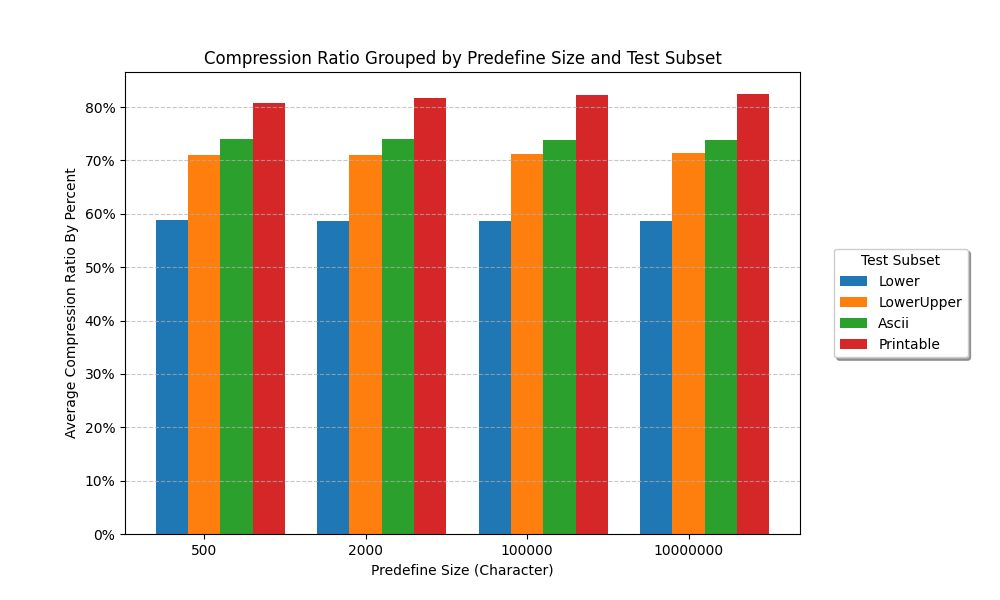
\includegraphics[width=1\linewidth]{total.png}
    \caption{Compression Ratio Group by File size and Character set}
    \label{fig:Compression-Ratio}
\end{figure}
\begin{itemize}
    \item This graph is presented as part of the experimental evaluation of a Huffman coding implementation. It visually summarizes the compression performance achieved across different input file sizes and character sets. The y-axis represents the "\textbf{Average Compression Ratio By Percent}" which we'll define precisely below. The x-axis groups the results by "\textbf{Predefined Size by Character}" representing the total number of characters in the input files. Within each size group, there are four bars, each representing a different "\textbf{Test Subset}" (character set).
    \item The compression ratio is calculated using the formula: 
\[Compression Ratio = (Encoded File Size / Original File Size) * 100\%\]
\textbf{A lower compression ratio is better}, indicating a greater reduction in file size. A ratio of 100\% means that there are no compression; a ratio of 50\% indicate that the encoded file is half the size of the original. A ratio above 100\% would imply that the "\textbf{compressed}" file is actually larger than the original (which is possible with Huffman coding if the input data has a very uniform distribution of characters).
    \item The graph shows four distinct file size groups: 500, 2000, 100000 and 10000000 characters. Within each character set, the compression ratio remains consistent across these different file sizes. This suggests the effectiveness of Huffman Coding is largely \textbf{independent of overall file size}. 
    \item \textbf{The strong dependence of the compression ratio on the character set is directly due to the structure of the Huffman tree}. Larger character sets, particularly those with many low-frequency characters, result in taller trees and longer average code lengths, decreasing the compression efficiency.
\end{itemize}
\subsection{Conclusion}
These results confirm that Huffman Coding is an effective lossless compression technique for ASCII text files. Under standard conditions (Printable character set), Huffman Encoding reduces file size by approximately 20\%. In specific cases, such as datasets with highly repetitive characters, the reduction can be as high as 30\%.
\newpage

\section{Advantage and disadvantage of the Static Huffman Coding}
\subsection{Advantages}
\begin{itemize}
    \item Huffman Coding using the probability of the symbol, helps produce an optimal prefix code. The code generated is guaranteed to be the lowest average code length for this specific distribution.
    \item Huffman Coding is a lossless encoding technique, guaranteeing the data is intact after decode.
    \item Huffman Coding has a relatively simple implementation.
    \item Huffman Coding is widely used and supported (JPEG, MP3, DEFLATE)
    \item Decoding a Huffman encoded code is generally very fast since it only needs to traverse the Huffman Tree.
\end{itemize}
\subsection{Disadvantages}
\begin{itemize}
    \item Require a prior knowledge of the data (frequencies) to build Huffman Tree to encode input.
    \item Huffman Coding is not adapted, if the frequencies slightly differ from the start the compression ratio will be suboptimal.
    \item The overhead of storing the Huffman Tree is also a problem.
    \item Huffman Coding treats each symbol independently, so it can’t take advantage of correlations between symbols ("q" is almost always followed by "u").
    \item Can be inefficient for super large character sets as already shown in the IO section.
    \item Vulnerable to Bits error. A single bit change can resolve the whole decoded text being wrong since Huffman Coding does not have an error correction part.
\end{itemize}
\newpage

\section{Discover the Application of Algorithm}
Huffman coding is a fundamental of lossless data compression so it is applied in various fields such as File Compression, Multimedia Compression, Data Transmission and Networking, Artificial Intelligence and Machine Learning, Hardware and Embedded Systems.
\begin{enumerate}[label=\textbf{\Alph*.}]
    \item \textbf{File Compression}
    \begin{itemize}
    \item Huffman coding is a common algorithm used in file compression because it helps to reduce file size without losing information.
    \item For example:
        \begin{itemize}
            \item 7-Zip: a popular open-source program for archiving files. It uses Deflate compression which is a combination of LZ77 and Huffman coding.
            \item WinZip and WinRAR: These are commercial file archiving tools that also use DEFLATE compression, including Huffman coding.
            \item macOS Archive Utility (built-in .zip functionality): The built-in archive utility in macOS creates and extracts ZIP files and it relies on DEFLATE.
            \item Command-line tools (gzip, zip): common tools found in Unix-like systems (Linux, macOS), their primary compression method is Deflate.
        \end{itemize}
    \end{itemize}
    \item \textbf{Multimedia Compression}
    \begin{itemize}
    \item Huffman coding is also used in compressing images, audio, and video. The \\algorithm can reduce file sizes while maintaining quality.
    \item For example:
        \begin{itemize}
            \item JPEG (Image Compression): It uses Huffman coding to compress pixel data after Discrete Cosine Transform (DCT).
            \item MP3 (Audio Compression): Huffman coding is used to compress quantized frequency data. It helps to reduce redundancy in audio streams.
            \item MPEG-4 (Video Compression): Huffman coding is used to compress motion vector data in video frames.
        \end{itemize}
    \end{itemize}
    \item \textbf{Data Transmission and Networking}
    \begin{itemize}
    \item By reducing the amount of data sent over the internet, Huffman coding helps to improve network efficiency.
    \item For example:
        \begin{itemize}
            \item HTTP Content-Encoding (GZIP): Web servers use GZIP which includes Huffman coding to compress CSS, HTML, and Javascript files and speed up web loading times.
            \item Fax Machines and Telephony: They use Group 3 fax encoding which includes Huffman coding to compress text-based data for faster transmission. 
        \end{itemize}
    \end{itemize}
    \item \textbf{Artificial Intelligence and Machine Learning}
    \begin{itemize}
    \item Huffman coding is applied in these fields for efficient memory usage.
    \item For example:
        \begin{itemize}
            \item Decision Tree Compression: optimize large decision trees in machine learning.
            \item Natural Language Processing (NLP): Huffman coding is applied in dictionary-based text compression for language modeling.
        \end{itemize}
    \end{itemize}
    \item \textbf{Hardware and Embedded Systems}
    \begin{itemize}
    \item To compress real-time data, hardware chips, and embedded devices need to implement Huffman coding.
    \item For example:
        \begin{itemize}
            \item GPUs and FPGAs: real-time compression in high-performance computing (HPC).
            \item Data Storage Systems: reduce file size in SSDs and HDDs.
        \end{itemize}
    \end{itemize}
\end{enumerate}
\newpage

\section{Compare with other Compression Algorithms}
\subsection{Introduce}
Huffman Coding is a solid foundation for data compression. While being fundamental, its performance and suitability must be evaluated against other lossless compression algorithms to have a clear picture of the world of compression algorithms. This section provides a comprehensive comparison between Huffman Coding and other significant lossless compression algorithms, especially RLE (Run-Length Encoding), Arithmetic Coding, and the Lempel-Ziv (LZ) family of methods. This evaluation will primarily focus on key performance metrics, including compression efficiency, computational complexity (encoding/decoding speeds), adaptability to varying data characteristics, and associated overhead.\newline
Let's assume that \(N\) represents the length of the input data and \(M\) speaks for the size of the character set.
\subsection{Huffman Coding vs RLE}
\begin{table}[H]
    \centering
    \renewcommand{\arraystretch}{1.5}
    \setlength{\tabcolsep}{8pt} % Giảm khoảng cách giữa các cột để tiết kiệm không gian
    \rowcolors{2}{gray!15}{white}
    \begin{tabular}{|p{0.15\linewidth}|p{0.35\linewidth}|p{0.35\linewidth}|}
        \hline
        \rowcolor{gray!30}
        \textbf{Feature} & \textbf{Huffman Coding} & \textbf{Run-Length Encoding(RLE)}\\
        \hline
        Principle & Variable-length codes based on symbol frequencies. & Replaces repeated substrings with references.\\\hline
        Complexity & Time:   O(N + M log M). \newline Space: O(M). &Time:   O(N). \newline Space: O(N).\\\hline
        Adaptivity & Static version is not adaptive; adaptive versions exist but are more complex. & Not inherently adaptive.\\\hline
        Overhead & Requires storing the Huffman tree (or frequencies) to decode. & Minimal overhead (just the counts).\\\hline
        Use Cases & General-purpose compression, JPEG, MP3, GZIP. & Simple images (e.g., fax), data with long runs.\\\hline
        Strengths & Good overall compression, widely supported. & Very fast and simple for suitable data.\\\hline
        Weaknesses & Can’t take advantage of correlations betweens symbols. & Poor compression for data without long runs.\\\hline
    \end{tabular}
    \caption{Huffman Coding vs RLE}
    \label{tab:Huffman_vs_RLE}
\end{table}
\subsection{Huffman Coding vs Arithmetic Coding}  
\begin{table}[H]  
    \centering  
    \renewcommand{\arraystretch}{1.5} % Giảm khoảng cách giữa các dòng  
    \setlength{\tabcolsep}{8pt} % Giảm khoảng cách giữa các cột  
    \rowcolors{2}{gray!15}{white}   
    \begin{tabular}{|p{0.15\linewidth}|p{0.35\linewidth}|p{0.35\linewidth}|}  
    \hline  
    \rowcolor{gray!30}  
        \textbf{Feature} & \textbf{Huffman Coding} & \textbf{Arithmetic Coding}\\\hline  
        Principle & Variable-length codes based on symbol frequencies. & Encodes the entire message as a single fraction.\\\hline  
        Complexity & Time:   O(N + M log M). \newline Space: O(M). & Time: O(N + M). \newline Space: O(M).\\\hline  
        Adaptivity & Static version is not adaptive; adaptive versions exist but are more complex. & Can be easily made adaptive. \\\hline  
        Overhead & Requires storing the Huffman tree (or frequencies) to decode. & Minimal overhead (typically just model parameters).\\\hline  
        Use Cases & General-purpose compression, JPEG, MP3, GZIP. & JPEG 2000, JBIG2, high-performance compression.\\\hline  
        Strengths & Good overall compression, widely supported. & Better compression, especially for small alphabets.\\\hline  
        Weaknesses & Can’t take advantage of correlations between symbols. & More complex, slower encoding/decoding.\\\hline  
    \end{tabular}  
    \caption{Huffman Coding vs Arithmetic Coding}  
    \label{tab:Huffman_vs_Arithmetic}  
\end{table}  

\subsection{Huffman Coding vs Lempel-Ziv Algorithms (LZ77, LZ78, LZW)}  
\begin{table}[H]  
    \centering   
    \renewcommand{\arraystretch}{1.5} % Giảm khoảng cách giữa các dòng  
    \setlength{\tabcolsep}{8pt} % Giảm khoảng cách giữa các cột  
    \rowcolors{2}{gray!15}{white}  
    \begin{tabular}{|p{0.15\linewidth}|p{0.35\linewidth}|p{0.35\linewidth}|}  
    \hline  
    \rowcolor{gray!30}  
        \textbf{Feature} & \textbf{Huffman Coding} & \textbf{Lempel-Ziv Algorithms}\\\hline  
        Principle & Variable-length codes based on symbol frequencies. & Replaces repeated substrings with references. \\\hline  
        Complexity & Time:   O(N + M log M). \newline Space: O(M). & Time: O(N). \newline Space: O(N).\\\hline  
        Adaptivity & Static version is not adaptive; adaptive versions exist but are more complex. & Adaptive, learns patterns in the data. \\\hline  
        Overhead & Requires storing the Huffman tree (or frequencies) to decode. & Minimal overhead (dictionary is built dynamically).\\\hline  
        Use Cases & General-purpose compression, JPEG, MP3, GZIP. & GZIP, ZIP, PNG (LZ77 + Huffman), GIF (LZW).\\\hline  
        Strengths & Good overall compression, widely supported. & Good for data with repeating patterns, adaptive.\\\hline  
        Weaknesses & Can’t take advantage of correlations between symbols. & Can be slower than Huffman.\\\hline  
    \end{tabular}  
    \caption{Huffman Coding vs Lempel-Ziv Algorithms}  
    \label{tab:Huffman_vs_Lempel-Ziv}  
\end{table}  
\subsection{Huffman Coding vs Burrows-Wheeler Transform (BWT)}  
\begin{table}[H]  
    \centering  
    \renewcommand{\arraystretch}{1.5} % Giảm khoảng cách giữa các dòng  
    \setlength{\tabcolsep}{8pt} % Giảm khoảng cách giữa các cột  
    \rowcolors{2}{gray!15}{white}   
    \begin{tabular}{|p{0.15\linewidth}|p{0.35\linewidth}|p{0.35\linewidth}|}  
    \hline  
        \rowcolor{gray!30}  
        \textbf{Feature} & \textbf{Huffman Coding} & \textbf{Burrows-Wheeler Transform}\\\hline  
        Principle & Variable-length codes based on symbol frequencies. & Reorders data to group similar characters together. Not a compression algorithm itself, but a preprocessor.\\\hline  
        Complexity & Time: O(N + M log M). \newline Space: O(M). & Time: O(N log N) \newline Space: O(N).\\\hline  
        Adaptivity & Static version is not adaptive; adaptive versions exist but are more complex. & Not applicable. \\\hline  
        Overhead & Requires storing the Huffman tree (or frequencies) to decode. & Minimal overhead, needs to store the index of the original string.\\\hline  
        Use Cases & General-purpose compression, JPEG, MP3, GZIP. & bzip2\\\hline  
        Strengths & Good overall compression, widely supported. & Very high compression ratio, especially for text.\\\hline  
        Weaknesses & Can’t take advantage of correlations between symbols. & Relatively slow.\\\hline  
    \end{tabular}  
    \caption{Huffman Coding vs Burrows-Wheeler Transform}  
    \label{tab:Huffman_vs_BWT}  
\end{table}  
\subsection{Conclusion}
There are no perfect compression algorithms, the performance of these compression algorithms is heavily dependent on the input data and specific requirements (compression ratio, speed, memory usage, etc.). Huffman Coding is a versatile and widely used technique, often used with other algorithms to create a more complex compression scheme (JPEG, GZIP, DEFLATE).
\newpage

\nocite{*}
\printbibliography[]
\end{document}